\documentclass[times, utf8, diplomski]{fer}
\usepackage{booktabs}
\usepackage{pdfpages}
\usepackage{listings}

\renewcommand{\lstlistingname}{Isječak}

\lstset{
	basicstyle=\linespread{1.2}\ttfamily\footnotesize,
	keepspaces=true,
	numbers=left,
	frame=single,
	captionpos=b,
	showspaces=false,
	numberstyle=\ttfamily,
	columns=flexible,
	extendedchars=true,
	inputencoding=utf8,
	xleftmargin=5mm,
	xrightmargin=5mm
}

\begin{document}

\thesisnumber{2565}

\title{Analiza performansi sustava za udaljeno izvršavanje programskog kôda}

\author{Herman Zvonimir Došilović}

\maketitle

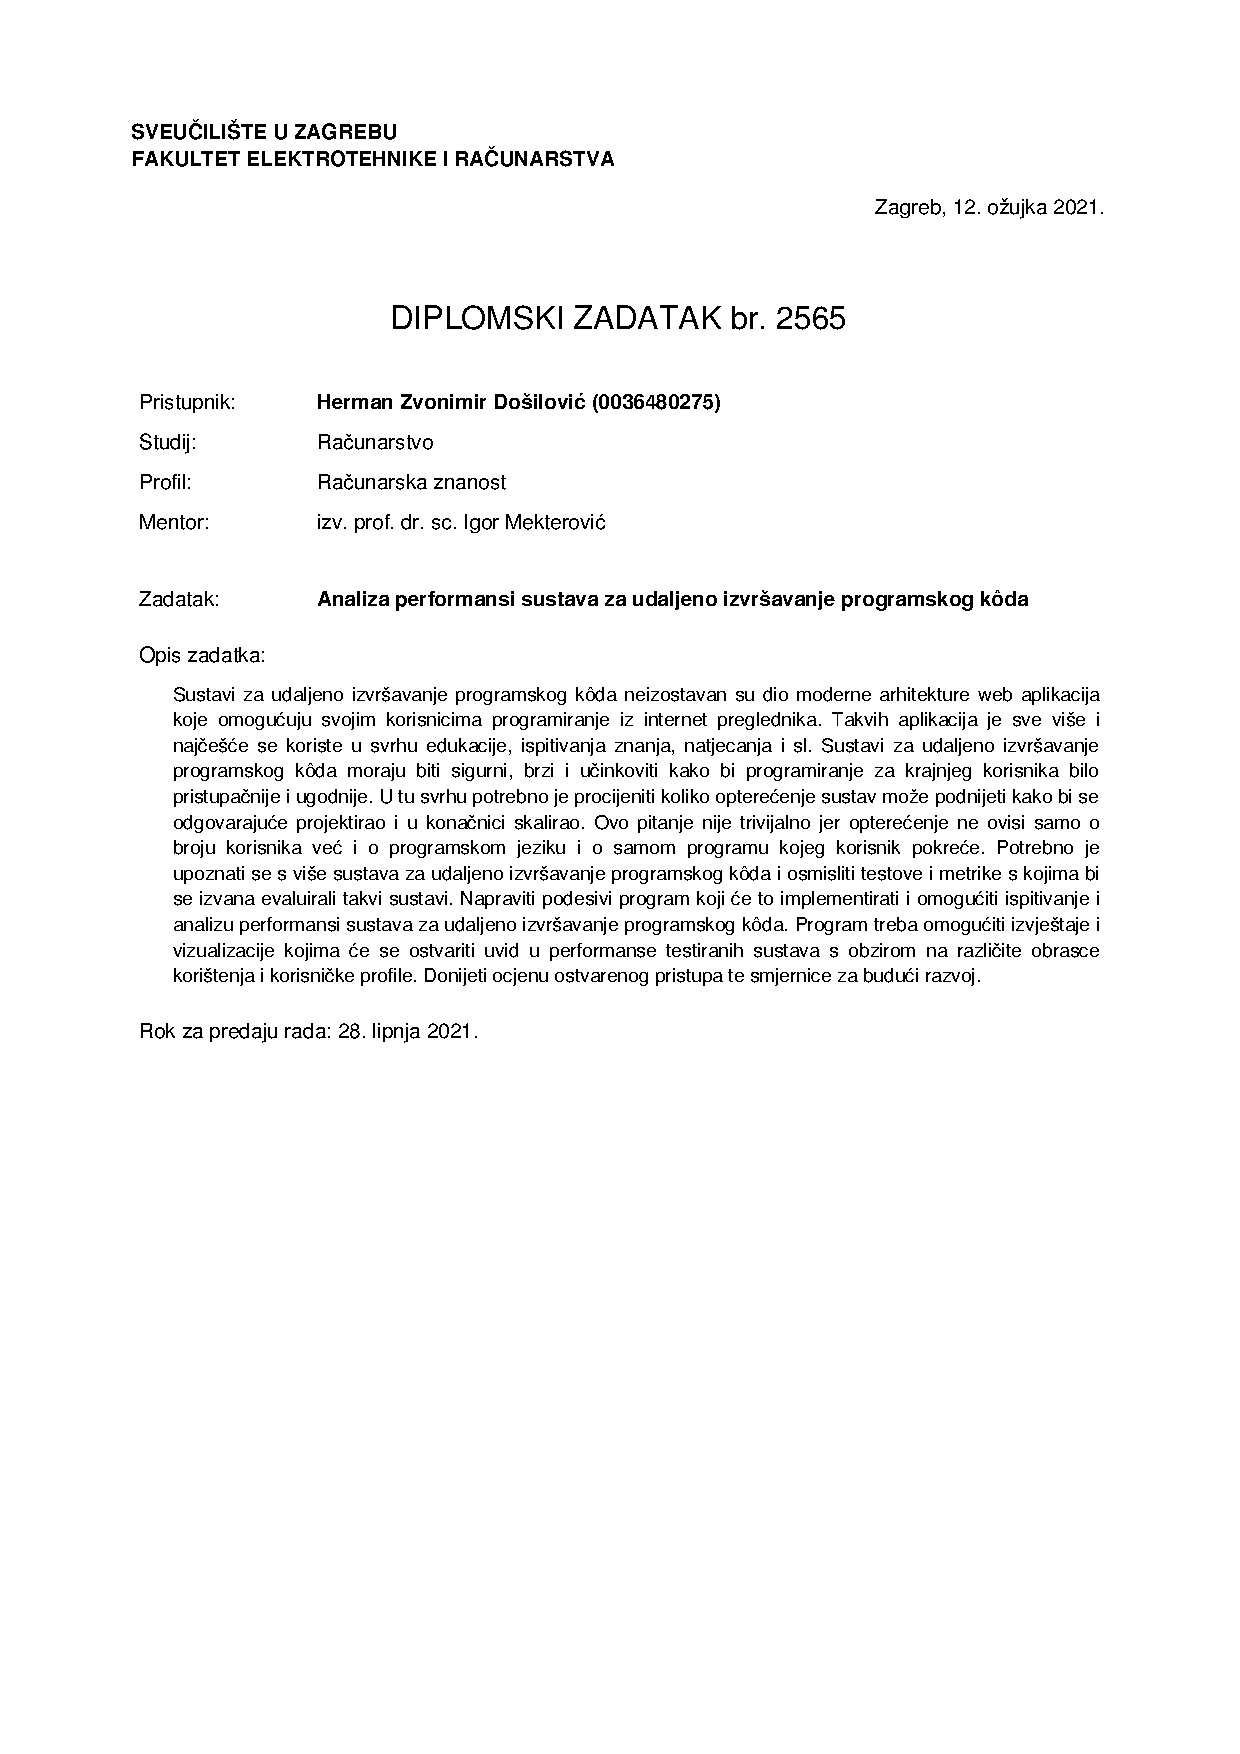
\includepdf[pages=-]{hr_0036480275_56.pdf}

\zahvala{}

\tableofcontents

\chapter{Uvod}
Računarsko razmišljanje \engl{computational thinking} je termin kojeg je prvi put upotrijebio Seymour Aubrey Papert 1980.\ godine u svojoj knjizi \textit{Mindstorms: Children, Computers, and Powerful Ideas} \citep{10.5555/1095592} u kojoj, između ostalog, razmatra korištenje računala kao alata koji može utjecati na način na koji ljudi uče i razmišljaju. Njegova vizija korištenja računala u edukaciji djece bila je naučiti djecu programirati računalo s ciljem da djeca već u ranoj dobi dotaknu neke od najdubljih ideja iz raznih znanstvenih disciplina. Papert programiranje računala opisuje kao komunikaciju između čovjeka i računala jezikom koji oboje razumiju, i time je njegova ideja razvoja računala, s kojim je prirodno naučiti  komunicirati, temeljna ideja koja se provlači kroz cijelu knjigu. Njegove ideje i inovacije promijenile su način na koji milijuni djece stvaraju i uče \citep{Papert.MITMediaLab}.

Termin \textit{računarsko razmišljanje} ponovo dobiva značajnu pažnju akademske zajednice \citep{grover2013computational} 2006.\ godine objavom istoimenog rada Jeannette M.\ Wing  koja računarsko razmišljanje svrstava u fundamentalnu vještinu pored čitanja, pisanja i aritmetike \citep{wing2006computational}. Njezin je rad potaknuo intenzivnije istraživanje o važnosti uključivanja računarskog razmišljanja u edukacijski sustav \citep{lockwood2017computational}. U svom izvješću iz 2014.\ godine internacionalna neprofitna organizacija European Schoolnet prepoznala je važnost integracije računarskog razmišljanja u edukacijski sustav te navode da već tada programiranje počinje biti sve ključnija vještina koju će morati steći svi mladi, ali i radnici iz širokog spektra industrije \citep{balanskat2014computing}. Navode, također, da je programiranje dio logičkog rasuđivanja i da ono pripada ključnim vještinama 21.\ stoljeća, što dodatno potkrjepljuje ideje Jeannette M.\ Wing iz 2006.\ godine.

Programiranje je od 2015.\ godine uključeno u nastavni plan i program 16 Europskih zemalja koje kod svojih učenika žele razviti vještine logičkog razmišljanja i rješavanja problema, ali i povećati mogućnost zapošljavanja \citep{balanskat2015computing}. Budući da se vještina programiranja stječe vježbanjem \citep{kurnia2001online}, institucije, koje u svom nastavnom planu i programu nude programiranje, svojim studentima trebaju omogućiti pristup biblioteci problemskih zadataka. Programska rješenja studenata konačno netko treba i ocijeniti, a tradicionalno ručno ocjenjivanje programskog kôda unosi dodatne probleme \citep{kurnia2001online}.

Probleme koje unosi tradicionalno ručno ocjenjivanje programskog kôda rješavaju \textbf{sustavi za udaljeno ocjenjivanje} (engl.\ \textit{online judges}, krat.\ \textit{OJs}) koji poboljšavaju proces edukacije i ocjenjivanja, ali i omogućuju studentima da prevedu \engl{compile} i izvrše \engl{execute} svoj programski kôda prije predaje \citep{wang2021metaoj}. Sustavi za udaljeno ocjenjivanje, poput \textit{web} aplikacije Edgar \citep{mekterovic2020building} razvijene na Fakultetu elektrotehnike i računarstva Sveučilišta u Zagrebu, omogućuju nastavnicima izradu \textit{online} provjera znanja koje pomoću ispitnih primjera automatski ocjenjuju rješenja studenata predana u obliku programskog kôda i time ubrzavaju proces ispravljanja i ocjenjivanja, i smanjuju mogućnost uvođenja grešaka koje se mogu dogoditi prilikom ručnog ocjenjivanja. Također, sustavi za udaljeno ocjenjivanje omogućuju studentima brzi pristup problemskim zadacima koje mogu rješavati i time vježbati svoju vještinu programiranja. Sustavi za udaljeno ocjenjivanje najčešće omogućuju studentima programiranje u pregledniku odnosno kroz \textit{web} aplikaciju koju koristi njihova institucija. Mogućnost programiranja i predaje rješenja kroz \textit{web} aplikaciju olakšava studentima, pogotovo početnicima, proces postavljanja okoline za programiranje u programskom jeziku koji pokriva nastavni plan i program koji pohađaju.

Jasno je dakle da se programski kôd studenta ne može prevesti i izvršiti direktno na njegovom računalu budući da na njemu nema postavljenju okolinu koja to omogućuje. Programski kôd studenta kojeg piše u svom pregledniku izvršava se na poslužitelju sustava za udaljeno ocjenjivanje. Sustav za udaljeno ocjenjivanje, poput već spomenute \textit{web} aplikacije Edgar, oslanja se na \textbf{sustav za udaljeno izvršavanje programskog kôda} (engl.\ \textit{online code execution system}, krat.\ \textit{OCES}) koji mu osigurava da će se programski kôd studenta prevesti i izvršiti bez negativnih posljedica za poslužitelj i ostalih korisnika aplikacije. Stoga OCES predstavlja ključnu komponentu u arhitekturi sustava za udaljeno ocjenjivanje o kojoj ovisi prije svega sigurnost i integritet poslužitelja, a zatim i korisničko iskustvo, i kvaliteta usluge.

Sustavi za udaljeno izvršavanje programskog kôda nude \textit{web} aplikacijsko sučelje koje sustavi za udaljeno ocjenjivanje mogu transparentno koristiti za stvaranje zahtjeva za izvršavanje programskog kôda, dohvat informacija o izvršavanju i dohvat rezultata izvršavanja. Sučelje koje takvi sustavi nude je jednostavno za korištenje, međutim, usluga koju nude je resursno i sigurnosno zahtjevna. Dobro izveden i skaliran sustav za udaljeno izvršavanje programskog kôda donosi veliku vrijednost sustavima za udaljeno ocjenjivanje budući da se razvojni inženjeri tih sustava tada mogu u potpunosti fokusirati na razvoj proizvoda i njegovih funkcionalnosti što krajnjem korisniku donosi bolje korisničko iskustvo i kvalitetniju uslugu.

Budući da se sustavi za udaljeno izvršavanje programskog kôda u literaturi razmatraju kao zasebne komponente arhitekture sustava za udaljeno ocjenjivanje tek od \citep{9245310}, ne postoji u literaturi radni okvir ocjene kvalitete i pouzdanosti takvih sustava. Kvaliteta i pouzdanost sustava za udaljeno izvršavanje programskog kôda dolazi do izražaja pri intenzivnom višekorisničkom opterećenju koje, u kontekstu sustava za udaljeno izvršavanje programskog kôda, predstavljaju zahtjevi za izvršavanje programskog kôda koje sustav dobiva kroz \textit{web} aplikacijsko sučelje.

Ovaj rad predstavlja prvi radni okvir za ocjenu kvalitete i pouzdanosti usluge koju nude sustavi za udaljeno izvršavanje programskog kôda. Ovaj rad također predstavlja i aplikaciju Hélory\footnote{Sv.\ Ivo Hélory (1253.\ -- 1303.), po kome je aplikacija dobila ime, zaštitnik je, između ostalog i sudaca \engl{judges}.} koja implementira predstavljeni radni okvir za ocjenu kvalitete i pouzdanosti za tri sustava za udaljeno izvršavanje programskog kôda: Sphere Engine, Piston i Judge0. Razvijen u obliku komandno-linijske aplikacije, Hélory nudi jednostavno pokretanje višekorisničkog opterećenja na željenom sustavu, a nakon eksperimenta Hélory će generirati i pohraniti izvještaj o pokrenutom eksperimentu koji sadrži detaljne informacije o svakom pojedinom zahtjevu za izvršavanje i grafički prikaz metrika od interesa za ocjenu kvalitete i pouzdanosti usluge.

U poglavlju \ref{chap:oj-ecosystem} opisana je arhitektura OJ ekosustava, dan je pregled slučajeva uporabe \engl{use-cases} i opisana je problematika udaljenog izvršavanja programskog kôda. Dodatno, poglavlje \ref{chap:oj-ecosystem} donosi formalnu definiciju OCES-a kroz funkcionalne i nefunkcionalne zahtjeve, i daje pregled sustava koje Hélory podržava. Poglavlje \ref{chap:analysis} predstavlja radni okvir za ocjenu kvalitete i pouzdanosti usluge OCES-a, dok poglavlje \ref{chap:helory} daje pregled funkcionalnosti razvijene aplikacije Hélory. U poglavlju \ref{chap:use} pokazuje se primjer korištenja aplikacije Hélory u analizi performansi sustava Piston i Judge0. Konačno, poglavlje \ref{chap:future} daje smjernice za budući razvoj radnog okvira i aplikacije Hélory.

\chapter{Arhitektura ekosustava sustava za udaljeno ocjenjivanje}
\label{chap:oj-ecosystem}
Sustavi za udaljeno ocjenjivanje dio su arhitekture OJ ekosustava prikazane na slici \ref{fig:oj-ecosystem}, a koja započinje zaštićenim okruženjem \engl{sandbox} koje osigurava sigurno prevođenje i izvršavanje programskog kôda korisnika na poslužitelju, i završava specijaliziranim izvedbama sustava za udaljeno ocjenjivanje koji se koriste u raznim slučajevima uporabe. Ovo poglavlje daje pregled svake komponente arhitekture OJ ekosustava i motivaciju za njezino korištenje.

\begin{figure}[htb]
	\centering
	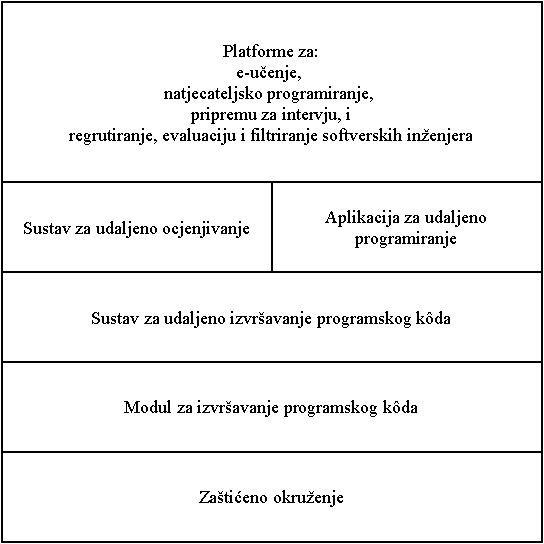
\includegraphics[width=0.75\textwidth]{images/Ekosustav.pdf}
	\caption{
		Arhitektura OJ ekosustava. \citep{9245310}
	}
	\label{fig:oj-ecosystem}
\end{figure}

\pagebreak

\section{Zaštićeno okruženje}
Sustavi za udaljeno ocjenjivanje koriste se za evaluaciju programskog kôda korisnika na unaprijed zadanom skupu primjera za ispitivanje, što povlači pitanje gdje će se programski kôd korisnika prevesti i izvršiti budući da se bez toga ne može ocijeniti njegovo rješenje. Najjednostavnije bi bilo da korisnik samostalno prevede i izvrši svoj program, i da zatim u sustav postavi rješenja koja je dobio. Ovakav pristup bio bi u redu za napredne korisnike koji znaju instalirati i koristiti odgovarajući prevoditelj za odabrani programski jezik, međutim, za početnike bi ovakav pristup rezultirao jako lošim korisničkim iskustvom. Ovo naime nije jedini argument zašto nije dobro da korisnik samostalno prevodi, izvršava i postavlja rješenja svojih programa. Ispitni primjeri trebaju ostati nepoznati korisniku kako ih ne bi zloupotrijebio. Korisnik ne treba znati očekivani izlaz \engl{expected output} svog programa da bi ga zloupotrijebio, jer je za neke zadatke dovoljno imati standardni ulaz \engl{standard input} iz kojeg se lako dobije očekivani izlaz. Već se samo sa ovim snažno opravdanim zahtjevom može zaključiti da je programski kôd korisnika potrebno izvršiti na poslužitelju kojem korisnik nema pristup. Ovakav zahtjev otvara novi spektar problema koje je potrebno riješiti i koji su opisani u \citep{kurnia2001online}.

Pokretanje programskog kôda korisnika na udaljenom poslužitelju nameće izazov da se korisnikov program mora pokrenuti u zaštićenom okruženju kako ne bi negativno utjecao na rad poslužitelja i ostalih procesa. Postoje razne tehnike opisane u \citep{yi2014comparison} koje se koriste za izvršavanje programskog kôda u zaštićenom okruženju, i u kontekstu sustava za udaljeno ocjenjivanje od zaštićenog okruženja očekujemo sljedeće funkcionalnosti:
\begin{itemize}
    \item[$\bullet$] inicijalizaciju zaštićenog okruženja,
    \item[$\bullet$] mogućnost prenošenja programskog kôda korisnika u zaštićeno okruženje,
    \item[$\bullet$] prevođenje i izvršavanje programskog kôda u zaštićenom okruženju uz navođenje procesorskih i memorijskih ograničenja,
    \item[$\bullet$] prikupljanje standardnog izlaza \engl{standard output} programa i ostalih meta podatka o izvršavanju, i
    \item[$\bullet$] čišćenje \engl{cleanup} zaštićenog okruženja.
\end{itemize}

Sustavi Judge0 i Piston, o kojima će biti riječ nešto kasnije u ovom poglavlju, koriste Isolate \citep{marevs2012new} i Docker \citep{merkel2014docker} kao zaštićena okruženja za prevođenje i izvršavanje programskog kôda. Isolate i Docker oboje koriste kontrolne grupe \engl{control groups}, značajke sustava Linux koje omogućuju definiranje resursnih ograničenja pojedinog procesa. Odabir korištenja jednog, odnosno drugog zaštićenog okruženja ovisi, između ostalog, o preferencijama razvojnih inženjera.

Važnost korištenja zaštićenog okruženja koje osigurava da programski kôd korisnika ne šteti radu poslužitelja i ostalih procesa prikazuju isječci \ref{lst:infinite-compilation} i \ref{lst:fork-bomb} napisani u programskom jeziku C. 

Isječak \ref{lst:infinite-compilation} prikazuje ispravan C program koji uključuje uređaj pseudo-slučajnih brojeva sustava Linux. Budući da uređaj generira beskonačni slijed pseudo-slučajnih brojeva, uključivanje tog uređaja dovodi do beskonačnog vremena prevođenja. Ukoliko više korisnika napravi zahtjev za izvršavanjem ovakvog ili sličnog programa, na poslužitelju brzo dolazi do iscrpljivanja procesorskih i memorijskih resursa i time postaje neupotrebljiv. Iz ovog je jednostavnog primjera jasno da je proces prevođenja potrebno pokrenuti u zaštićenom okruženju koje će imati ograničene procesorske i memorijske resurse.

\begin{lstlisting}[
    caption={Ispravan C program s beskonačnim vremenom prevođenja.},
    label={lst:infinite-compilation},
    language=c
]
#include </dev/random>
int main() {
    return 0;
}
\end{lstlisting}

Izoliranje izvršavanja programskog kôda korisnika još je važnije od izolacije prevođenja, budući da je za zloupotrebu neizoliranog procesa prevođenja potrebno nešto više znanja o prevodiocima i programskom jeziku koji se koristi. Isječak \ref{lst:fork-bomb} prikazuje C program koji će beskonačno mnogo puta stvoriti novi proces, i svaki novostvoreni proces napravit će isto. Budući da se broj novostvorenih procesa može opisati eksponencijalnom funkcijom $f(x) = 2^x$, gdje je $x$ broj ponavljanja petlje, ovaj program naziva se \textit{fork bomb}. Dovoljno je da jedan korisnik pokrene ovakav program da se na poslužitelju iscrpe procesorski i memorijski resursi koji će ga učiniti neupotrebljivim.

\begin{lstlisting}[
    caption={C program s beskonačnim grananjem novih procesa.},
    label={lst:fork-bomb},
    language=c
]
#include <unistd.h>
int main() {
    while(1) {
        fork();
    }
    return 0;
}
\end{lstlisting}

Oba isječka potvrđuju da je u sustavima za udaljeno ocjenjivanje nužno koristiti zaštićeno okruženje koja će prevesti i izvršiti programski kôd svakog korisnika. 

Gledajući iz perspektive sustava za udaljeno ocjenjivanje svaki programski kôd korisnika smatra se opasnim za poslužitelj, stoga se u kontekstu sustava za udaljeno ocjenjivanje govori o nepouzdanom programskom kôdu \engl{untrusted source code} kojeg je potrebno prevesti i izvršiti.

\section{Modul za izvršavanje programskog kôda}
Modul za izvršavanje programskog kôda (engl.\ \textit{code execution engine}, krat.\ \textit{CEE}) iduća je komponenta u arhitekturi OJ ekosustava koja koristi zaštićeno okruženje za prevođenje i izvršavanje programskog kôda, i koja zatim obrađuje meta podatke o prevođenju i izvršavanju koje generira zaštićeno okruženje. Slika \ref{fig:cee-and-sandbox} prikazuje dijagram toga interakcije između modula za izvršavanje programskog kôda i zaštićenog okruženja.

\begin{figure}[htb]
	\centering
	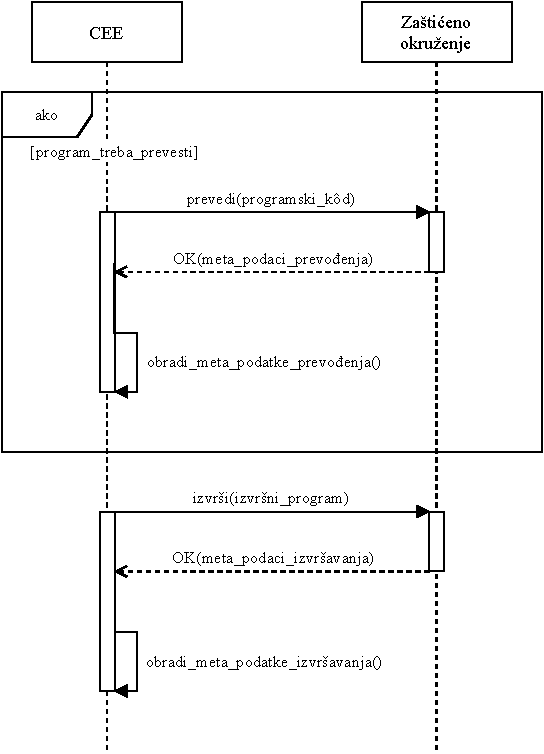
\includegraphics[width=0.65\textwidth]{images/CEE i zaštićeno okruženje.pdf}
	\caption{
		Interakcija modula za izvršavanje programskog kôda s zaštićenim okruženjem.
	}
	\label{fig:cee-and-sandbox}
\end{figure}

\pagebreak

\section{Sustav za udaljeno izvršavanje programskog kôda}
Sustav za udaljeno izvršavanje programskog kôda je sustav koji nudi \textit{web} aplikacijsko sučelje \engl{web API} za prevođenje i izvršavanje proizvoljnog programskog kôda. Arhitekturalni prikaz na slici \ref{fig:oj-ecosystem} izdvaja sustav za udaljeno izvršavanje programskog kôda kao zasebnu komponentu na koju se oslanjaju sustav za udaljeno ocjenjivanje, aplikacija za udaljeno programiranje, a zatim i specijalizirane izvedbe sustava za udaljeno ocjenjivanje razvijene za specifičan slučaj uporabe. Sustav za udaljeno izvršavanje programskog kôda najčešće je strogo povezan i zavisan o ostatku komponenata u arhitekturu sustava za udaljeno ocjenjivanje \citep{9245310}, međutim, u ovom radu razmatraju se oni sustavi za udaljeno izvršavanje programskog kôda koji su neovisni o ostatku arhitekture koja se na njih oslanja.

Slika \ref{fig:oces-architecture} prikazuje dijagram komponenti sustava za udaljeno izvršavanje programskog kôda koji preko \textit{web} aplikacijskog sučelja nudi uslugu izvršavanja programskog kôda (lijeva priključnica na slici \ref{fig:oces-architecture}) koju koriste sustav za udaljeno ocjenjivanje ili aplikacije za udaljeno programiranje. Putem OCES međuopreme \engl{middleware}, zahtjev za izvršavanje programskog kôda dolazi do modula za izvršavanje programskog kôda kojih u sustavu može biti više kako bi se prilikom intenzivnog višekorisničkog opterećenja zahtjevi za izvršavanje efikasnije obavili. Način izvedbe OCES međuopreme ovisi o pojedinom sustavu za udaljeno izvršavanje programskog kôda kao što se npr.\ međuoprema sustava Judge0 sastoji od PostgreSQL baze podataka koja pohranjuje sve zahtjeve za izvršavanje programskog kôda i rezultate prevođenja i izvršavanja, i Redis baze podataka koja se koristi kao red poslova \engl{job queue} \citep{9245310}.

Formalna definicija sustava za udaljeno izvršavanje programskog kôda dana je u \citep{9245310} kroz funkcionalne i nefunkcionalne zahtjeve. Funkcionalni zahtjevi podijeljeni su u nužne i dovoljne, odnosno na zahtjeve koje sustav nužno mora ispuniti i dodatne neobavezne zahtjeve. Nefunkcionalni zahtjevi su također neobavezni, ali preporučeni.

\begin{figure}[htb]
	\centering
	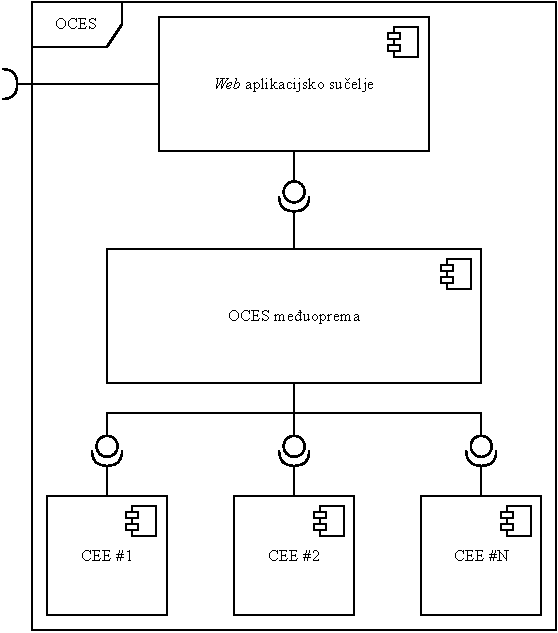
\includegraphics[width=0.75\textwidth]{images/Arhitektura OCES-a.pdf}
	\caption{
	    Dijagram komponenti sustava za udaljeno izvršavanje programskog kôda.
	}
	\label{fig:oces-architecture}
\end{figure}

\pagebreak

\subsubsection{Funkcionalni zahtjevi}
Sustav za udaljeno izvršavanje programskog kôda \textbf{mora} pružiti:
\begin{itemize}
    \item[$\bullet$] dobro dokumentirano \textit{web} aplikacijsko sučelje,
    \item[$\bullet$] podršku za prevođenje i izvršavanje proizvoljnog programskog kôda za barem jedan programski jezik,
    \item[$\bullet$] izvršavanje u zaštićenom okruženju s pretpostavljenim procesorskim i memorijskim ograničenjima,
    \item[$\bullet$] podršku za navođenje proizvoljnog standardnog ulaza, i
    \item[$\bullet$] podršku za dohvat rezultata izvršavanja programa koji sadrži barem standardni izlaz programa.
\end{itemize}

Dodatno, ali neobavezno, sustav za udaljeno izvršavanje programskog kôda \textbf{može} pružiti podršku za:
\begin{itemize}
    \item[$\bullet$] navođenje dodatnih opcija prevodioca,
    \item[$\bullet$] navođenje komandno-linijskih argumenata,
    \item[$\bullet$] navođenje resursnih ograničenja poput npr.\ procesorskih i memorijskih ograničenja,
    \item[$\bullet$] inicijalizaciju zaštićenog okruženja s dodatnim datotekama,
    \item[$\bullet$] dohvat detaljnih meta podataka o izvršavanju programa (npr.\ vrijeme izvođenja programa ili sadržaj standardnog izlaza za pogreške \engl{standard error}),
    \item[$\bullet$] skupne zahtjeve za izvršavanje,
    \item[$\bullet$] višestruke standardne ulaze, i
    \item[$\bullet$] autentifikaciju.
\end{itemize}

Čim više funkcionalnih zahtjeva sustav ispunjava tim više slučajeva uporabe može zadovoljiti. \citep{9245310}

\subsubsection{Nefunkcionalni zahtjevi}
Preporuča se da sustav za udaljeno izvršavanje programskog kôda bude:
\begin{itemize}
    \item[$\bullet$] skalabilan,
    \item[$\bullet$] konfigurabilan,
    \item[$\bullet$] siguran,
    \item[$\bullet$] lako upogonljiv,
    \item[$\bullet$] efikasan,
    \item[$\bullet$] otporan,
    \item[$\bullet$] proširiv, i
    \item[$\bullet$] robustan.
\end{itemize}

Čim više nefunkcionalnih zahtjeva sustav ispunjava tim ga je lakše integrirati u sustav specifično izveden za pojedini slučaj uporabe \citep{9245310}. Skalabilnost i efikasnost sustava za udaljeno izvršavanje programskog kôda dolazi do izražaja prilikom izrazitog višekorisničkog opterećenja kada krajnji korisnici neposredno preko sustava za udaljeno ocjenjivanje stvaraju zahtjeve za izvršavanje. Tada se od sustava za udaljeno izvršavanje programskog kôda očekuje da neovisno o broju zahtjeva efikasno izvrši programski kôd korisnika i vrati rezultate izvršavanja sustavu za udaljeno ocjenjivanje jer će u protivnom krajnje korisničko iskustvo biti srozano dugim vremenom čekanja. Konfigurabilnost i proširivost sustava za udaljeno izvršavanje programskog kôda omogućuje razvojnim inženjerima da sustav prilagode svojim zahtjevima prilikom razvoja sustava za određeni slučaj uporabe. Laka upogonljivost sustava za udaljeno izvršavanje programskog kôda omogućava razvojnim inženjerima da brzo napreduju u razvoju sustava za određeni slučaj uporabe. Sigurnost sustava za udaljeno izvršavanje programskog kôda uvelike ovisi načinu na koji sustav iskorištava funkcionalnosti zaštićene okoline i koristi li ju uopće. Od sustava se očekuje da niti jedan programski kôd ne naruši sigurnost i integritet poslužitelja. Ako se i dogodi da neki programski kôd uzrukuje neuobičajeno ponašanje, od sustava se očekuje da bude otporan i robustan na unutarnje pogreške koje se mogu dogoditi i da neovisno o njima vrati korisniku rezultat izvođenja.

U nastavku ove cjeline dan je pregled tri različita sustava za udaljeno izvršavanje programskog kôda koje podržava aplikacija Hélory.

\subsection{Sustav Sphere Engine}
Sustav za udaljeno izvršavanje programskog kôda Sphere Engine razvila je Poljska tvrtka Sphere Research Labs 2008.\ godine. Sphere Engine je jedan od vodećih komercijalnih sustava za udaljeno izvršavanje programskog kôda kojeg koristi više od 1000 institucija u 180 država. Jedna od najpoznatijih \textit{web} aplikacija koja koristi Sphere Engine je SPOJ \citep{SPOJ} koju je razvila ista tvrtka, a na kojoj korisnici mogu rješavati razne problemske zadatke iz domene natjecateljskog programiranja. Osim SPOJ-a, CodeChef \citep{CodeChef} također koristi Sphere Engine za udaljeno izvršavanje programskog kôda.

Budući da je Sphere Engine zatvoreni komercijalni sustav, nisu dostupne informacije o njegovoj izvedbi, niti o tome u kojim tehnologijama je razvijen.

U svrhu ovog rada dovoljno je spomenuti da sustav omogućuje prevođenje i izvršavanje programskog kôda u mnoštvo programskih jezika i da nudi bogatu dokumentaciju \textit{web} aplikacijskog sučelja.

\begin{figure}[htb]
	\centering
	
\includegraphics[width=\textwidth]{images/Sphere Engine Logo.png}
	\caption{
	    Vizualni identitet sustava Sphere Engine. \citep{SphereEngine}
	}
\end{figure}

\subsection{Sustav Piston}
Sustav za udaljeno izvršavanje programskog kôda Piston \citep{Piston} je sustav otvorenog kôda koji je dostupan na platformi GitHub. Razvijen je i koristi se u edukativne svrhe zajednice koju vodi autor projekta.

Kao zaštićeno okruženje u kojoj se izvršava programski kôda korisnika, sustav Piston koristi Docker i nudi oskudnu dokumentaciju \textit{web} aplikacijskog sučelja, međutim, kao i Sphere Engine, podržava mnoštvo programskih jezika koji se mogu koristiti. Zajednica koja razvija sustav Piston također je razvila i komandno-linijsku aplikaciju koja se povezuje sa sustavom i tako korisnicima omogućava da iz ljuske \engl{shell} pokrenu proizvoljni programski kôd, dobivajući tako privid da se njihov program izvršio izravno na njihovom računalu.

\begin{figure}[htb]
	\centering
	
\includegraphics[width=0.45\textwidth]{images/Piston Logo.png}
	\caption{
	    Vizualni identitet sustava Piston. \citep{Piston}
	}
\end{figure}

\pagebreak

\subsection{Sustav Judge0}
Razvoj sustava Judge0 započet je 22.\ kolovoza 2016.\ godine na inicijativu autora ovog rada. Cilj razvoja sustava Judge0 bio je izgradnja novog, robustnog, skalabilnog i lako uporabljivog sustava za udaljeno izvršavanje programskog kôda koji se može jednostavno integrirati u razne \textit{web} aplikacije koje trebaju funkcionalnost izvršavanja programskog kôda. Razvijen je u programskom jeziku Ruby koristeći radni okvir Ruby on Rails, a kao zaštićeno okruženje koristi Isolate \citep{marevs2012new} koji se također koristi u popularnom sustavu za udaljeno ocjenjivanje CMS \citep{maggiolo2012introducing}. Sustav CMS koristio se na najvećim međunarodnim natjecanjima iz natjecateljskog programiranja poput informatičke olimpijade (IOI) i srednjoeuropske informatičke olimpijade (CEOI) \citep{CMSWeb}. Akademskoj zajednici sustav Judge0 napokon je formalno predstavljen 2020.\ godine radom \citep{9245310}.

\begin{figure}[htb]
	\centering
	
\includegraphics[width=0.65\textwidth]{images/Judge0 Logo.png}
	\caption[]{
	    Vizualni identitet sustava Judge0.\footnotemark
	}
\end{figure}

\footnotetext{Vizualni identitet sustava Judge0 osmislio je i izradio Emanuel Loborec.}

U vrijeme pisanja ovog rada, javna instanca sustava Judge0 izvršila je preko 12,7 milijuna programa korisnika diljem svijeta koji su sustav Judge0 integrirali u svoje proizvode. Dodatno, u vrijeme pisanja ovog rada, zabilježeno je preko 200 aktivnih instanci sustava Judge0 kojeg su razne organizacije pokrenule na svojim poslužiteljima. 

Od akademske godine 2018./2019. sustav Judge0 aktivno se koristi na Fakultetu elektrotehnike i računarstva Sveučilišta u Zagrebu kao integracijski dio \textit{web} aplikacije Edgar \citep{mekterovic2020building}. Time je sustav Judge0, neposredno preko \textit{web} aplikacije Edgar, koristilo preko 3000 studenata kroz nekoliko predmeta.

Sustav Judge0 odlikuje se prije svega bogatom dokumentacijom \textit{web} aplikacijskog sučelja koje omogućuje jednostavno korištenje sustava s mnoštvo konfiguracijskih opcija. Obilje funkcionalnosti koje nudi Judge0 omogućuje razvojnim inženjerima laku integraciju s drugim sustavima raznih slučajeva uporabe.

\begin{figure}[htb]
	\centering
	
\includegraphics[width=\textwidth]{images/Judge0 Clients.png}
	\caption{
	    Vizualni identiteti organizacija koje koriste sustav Judge0. \citep{Judge0Web}
	}
	\label{fig:judge0-clients}
\end{figure}

\pagebreak

\section{Sustav za udaljeno ocjenjivanje}
Formalno, sustav za udaljeno ocjenjivanje \citep{wasik2018survey} definira kao udaljenu uslugu \engl{online service} koja u oblaku \engl{cloud} izvodi barem jednu od sljedećih faza:
\begin{itemize}
    \item podnošenje zahtjeva za izvršavanje programskog kôda \engl{submission},
    \item procjena podnesenoga programskog kôda \engl{assessment},
    \item ocjenjivanje podnesenoga programskog kôda \engl{scoring}.
\end{itemize}

Podnošenje zahtjeva za izvršavanje programskog kôda podrazumijeva prihvaćanje programskog kôda u sustav, prevođenje po potrebi i verifikaciju da je program spreman za izvršavanje. U procjeni podnesenoga programskog kôda program se pokreće za svaki ispitni primjer i provjerava se uspješnost izvođenja programa u zadanim procesorskim i memorijskim ograničenjima. Također, u istoj fazi, provjerava se standardni izlaz \engl{standard output} korisničkog programa i uspoređuje ga se s očekivanim izlazom za trenutni ispitni primjer \engl{expected output}. Konačno, u fazi ocjenjivanja, podnesenom programskom kôdu dodjeljuje se ocjena na temelju rezultata iz prethodnih faza. Tako npr.\ na ocjenu u natjecateljskom programiranju može utjecati vrijeme koje je bilo potrebno natjecatelju da riješi pojedini zadatak. Što kasnije natjecatelj riješi ispravno zadatak to će manje bodova dobiti čak i ako su mu svi ispitni primjeri ispravni uz zadana vremenska i memorijska ograničenja.

\section{Aplikacija za udaljeno programiranje}
Pored dosad nabrojanih specijaliziranih aplikacija koje se arhitekturalno oslanjaju na sustav za udaljeno ocjenjivanje (slika \ref{fig:oj-ecosystem}) postoje još i \textit{web} aplikacije za udaljeno programiranje \engl{online compilers} i \textit{web} aplikacije za udaljeno razvijanje \engl{online IDEs}. \textit{Web} aplikacija poput aplikacije Judge0 IDE \citep{Judge0IDE} u izvedbi aplikacije za udaljeno programiranje omogućuje korisniku pisanje, prevođenje i izvršavanje programskog kôda u jednom od podržanih programskih jezika (slika \ref{fig:judge0-ide-ui}). \citep{wasik2018survey} daje detaljnu usporedba ovakvih i sličnih \textit{web} aplikacija.

\begin{figure}[htb]
	\centering
	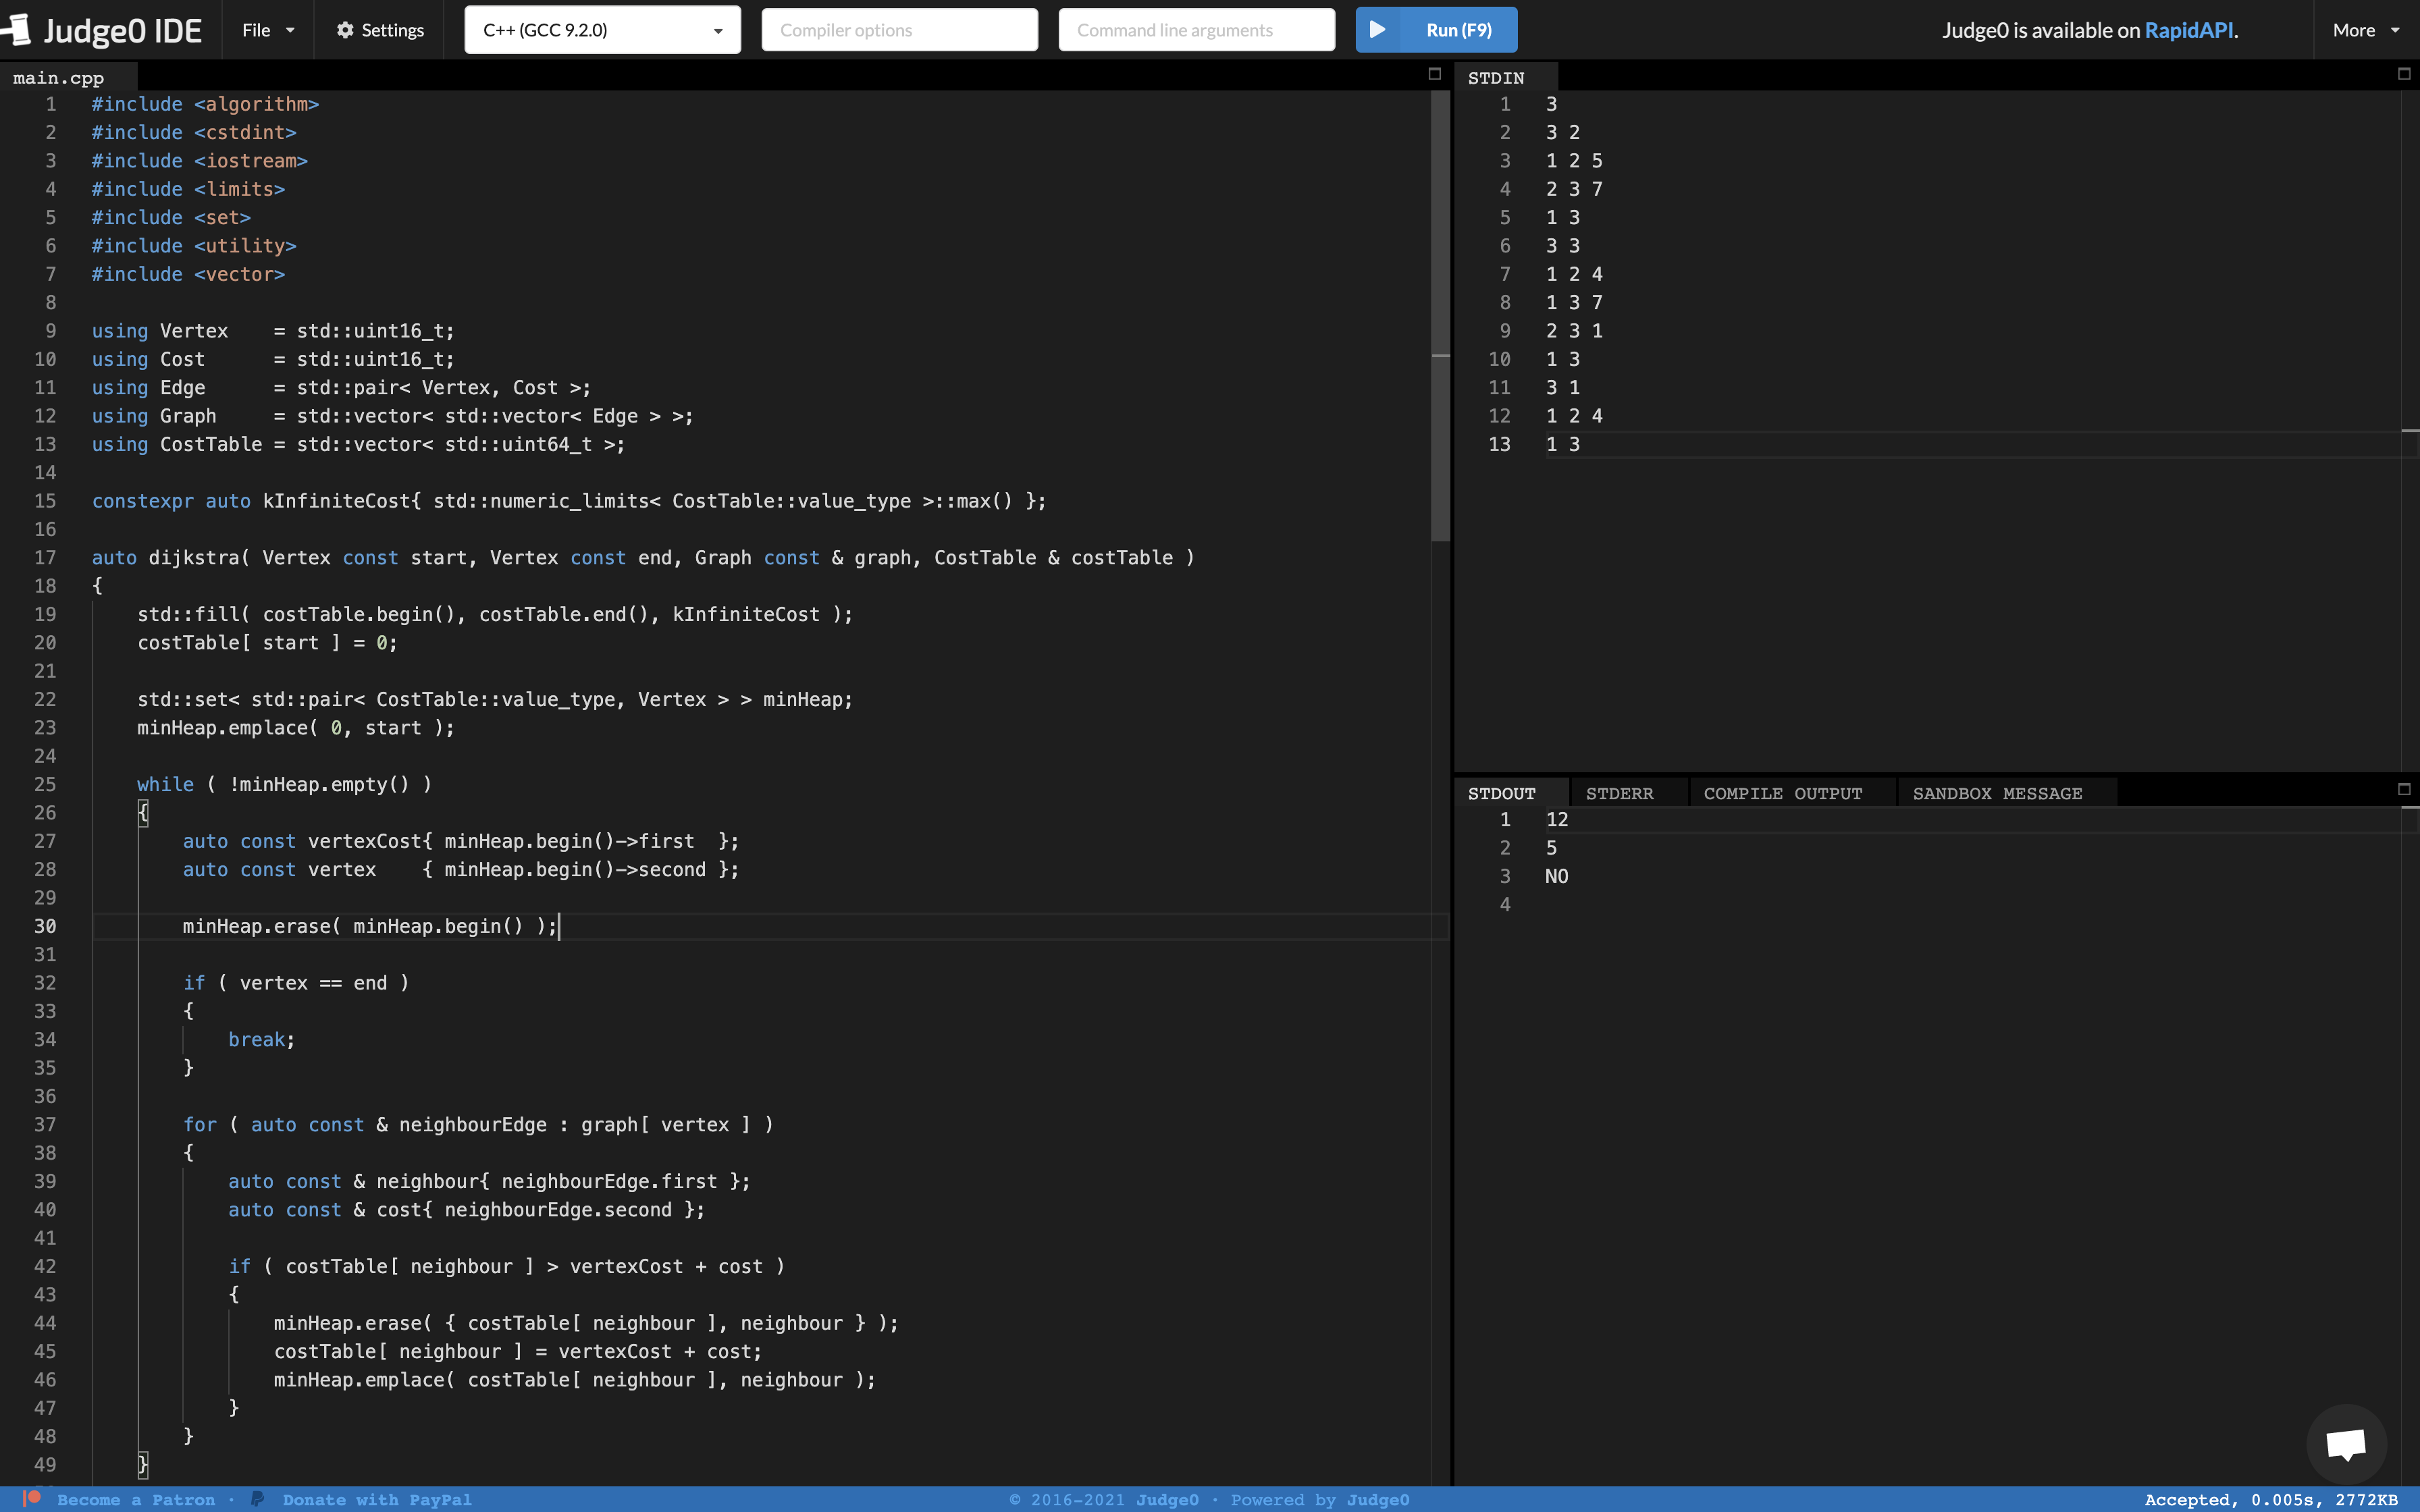
\includegraphics[width=\textwidth]{images/judge0-ide-ui.png}
	\caption{
		Sučelje \textit{web} aplikacije Judge0 IDE.
	}
	\label{fig:judge0-ide-ui}
\end{figure}

\section{Specijalizirane izvedbe sustava za udaljeno ocjenjivanje}
Najčešća izvedba sustava za udaljeno ocjenjivanje su \textit{web} aplikacije za natjecateljsko programiranje poput: Codeforces \citep{Codeforces}, CodeChef \citep{CodeChef} i SPOJ \citep{SPOJ} gdje se od korisnika očekuje da iz teksta zadatka prepozna i implementira algoritam i odgovarajuću strukturu podataka koji će zadovoljiti zadana vremenska i memorijska ograničenja. 

Izvedba sustava za udaljeno ocjenjivanje kao \textit{web} aplikacije za e-učenje poput \textit{web} aplikacija Edgar \citep{mekterovic2020building} i CodeChum \citep{maranga2019codechum} koristi se za ocjenjivanje \engl{scoring} programskog kôda kojeg student prilaže kao rješenje zadatka iz npr.\ domaće zadaće ili provjere znanja.

\begin{figure}[htb]
	\centering
	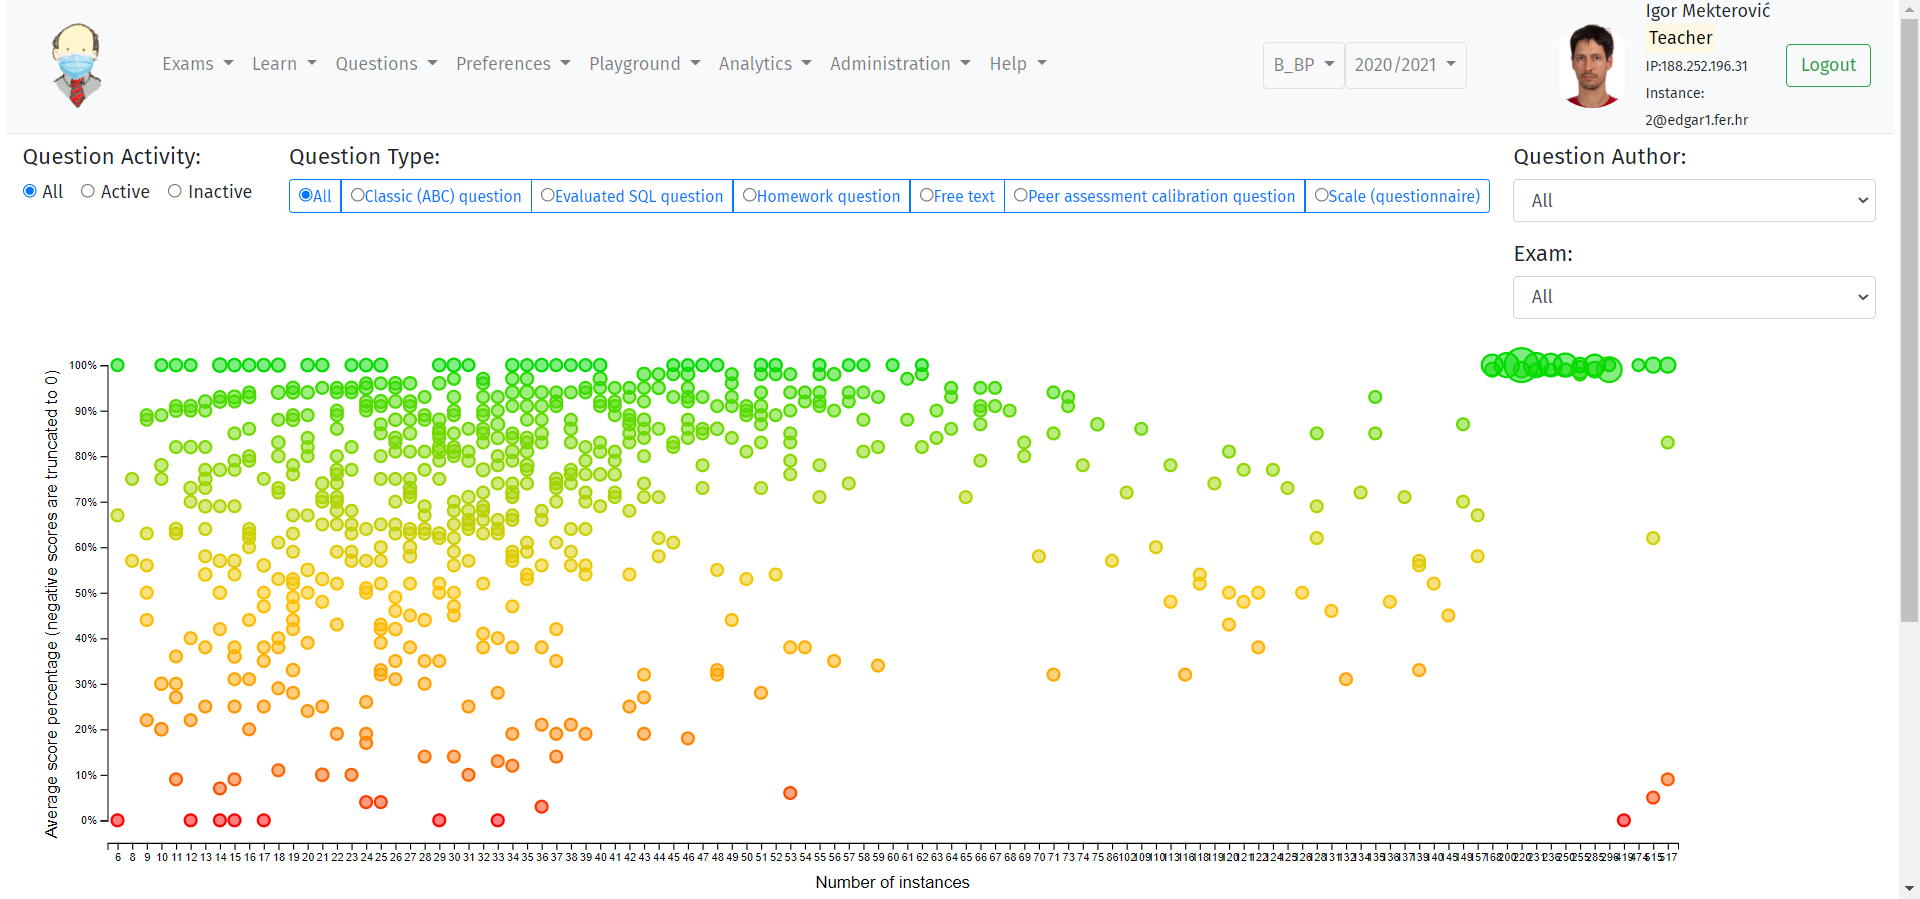
\includegraphics[width=\textwidth]{images/edgar-ui.png}
	\caption{
		Sučelje \textit{web} aplikacije Edgar iz perspektive učitelja.
	}
	\label{fig:edgar-ui}
\end{figure}

\begin{figure}[htb]
	\centering
	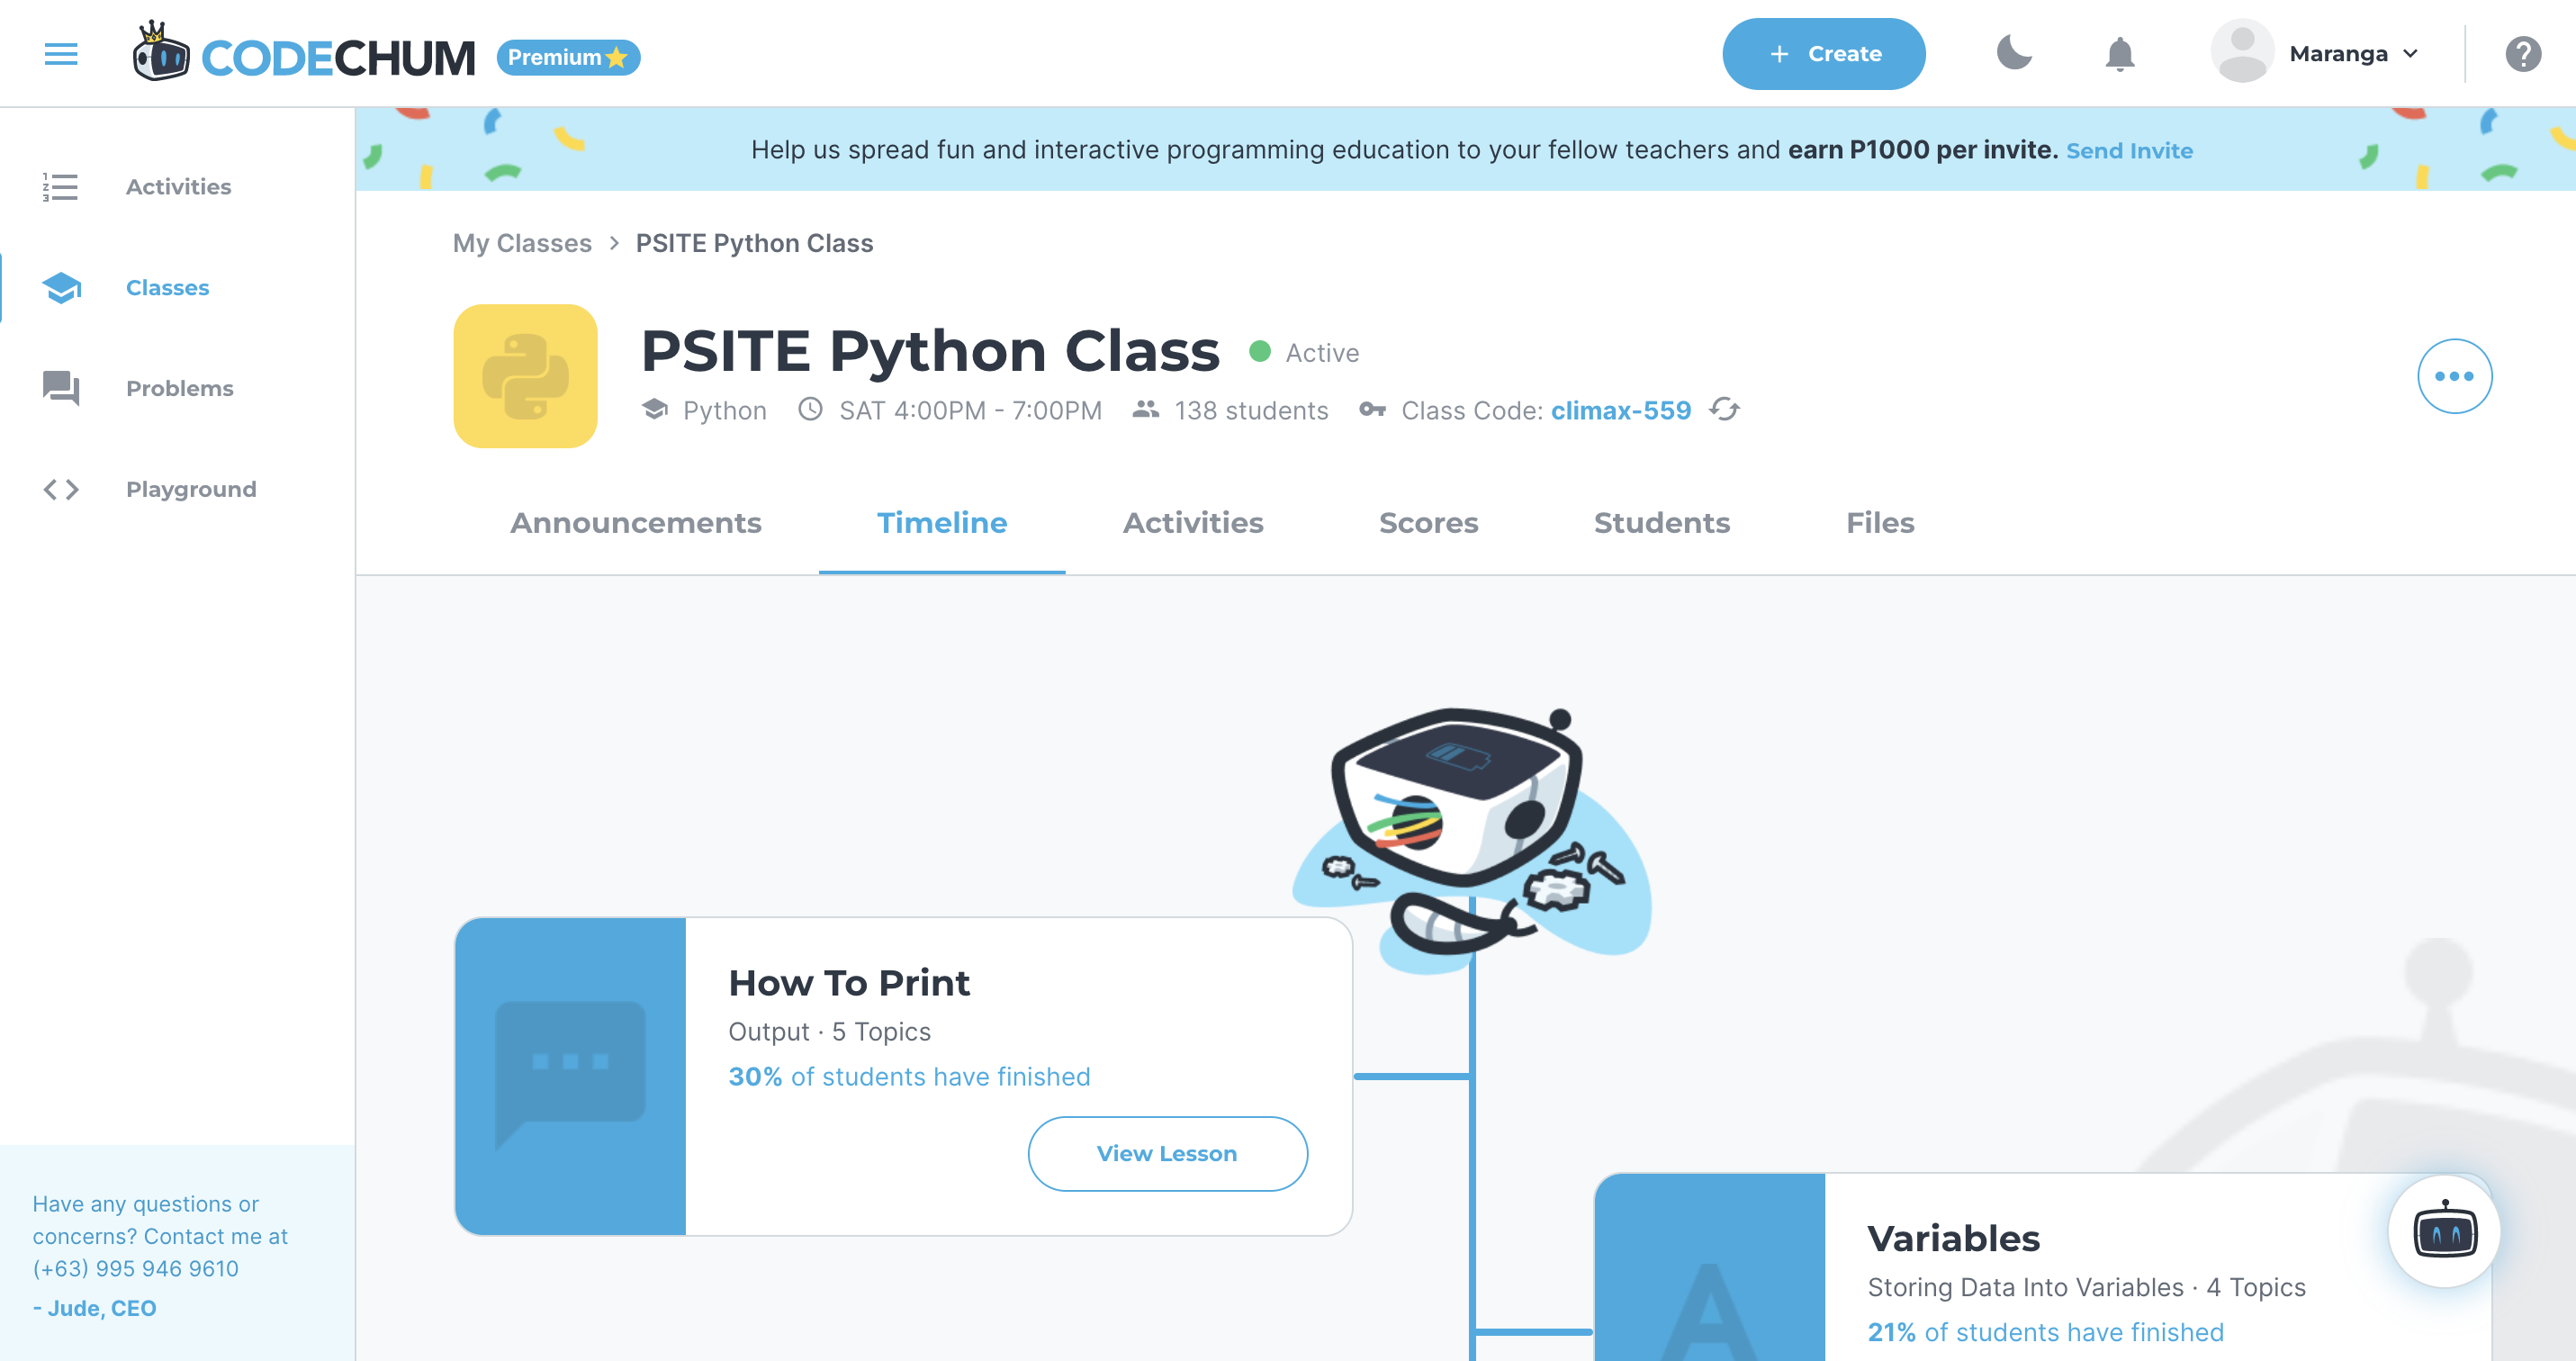
\includegraphics[width=\textwidth]{images/codechum-ui.png}
	\caption{
		Sučelje \textit{web} aplikacije CodeChum.
	}
	\label{fig:codechum-ui}
\end{figure}

\textit{Web} aplikacije poput HackerRank \citep{HackerRank}, TestDome \citep{TestDome} i Filtered \citep{Filtered} koriste se u regrutaciji i procesu zapošljavanja novih softverskih inženjera. Nakon što se prijave na otvorenu poziciju, kandidatima se automatski šalje elektronička pošta s uputama za rješavanje programskih zadataka. Zadatke koje će kandidat rješavati priprema tvrtka za čiju poziciju se kandidat natječe, a težina i vrsta zadataka ovisi o otvorenoj poziciji. Aplikacije za regrutaciju i automatizaciju procesa zapošljavanja najčešće nude svoju biblioteku zadataka koje tvrtke mogu odabrati prilikom izrade ispita za pojedini natječaj. Ovakve \textit{web} aplikacije korisne su tvrtkama koje svakodnevno dobivaju preveliku količinu prijava koje odjel za ljudske resurse može pogledati, stoga im automatizirano ispitivanje kandidata pomaže u inicijalnom filtriranju  prilikom zapošljavanja. Osim filtriranja kandidata ove \textit{web} aplikacije pomažu i pri provođenju \textit{online} razgovora gdje kandidati svoje vještine rješavanja problemskih zadatka trebaju pokazati pred ispitivačem koji vodi razgovor (slika \ref{fig:hackerrank-ui}).

\begin{figure}[htb]
	\centering
	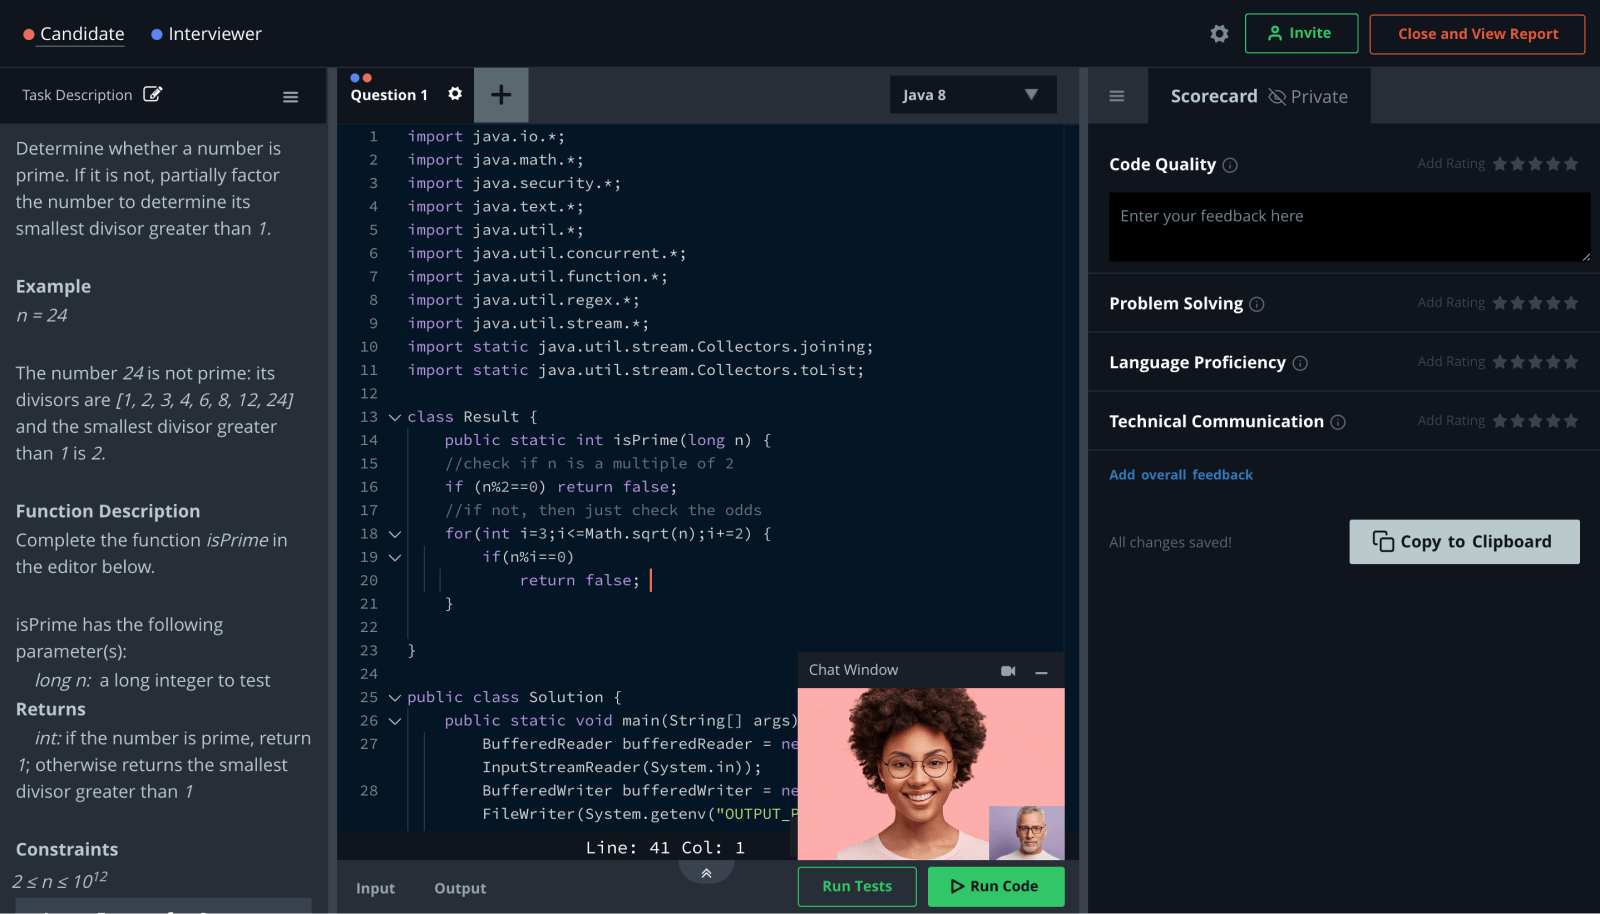
\includegraphics[width=\textwidth]{images/hackerrank-ui.png}
	\caption{
		Sučelje \textit{web} aplikacije HackerRank. \citep{HackerRank}
	}
	\label{fig:hackerrank-ui}
\end{figure}

Osim što pomažu u regrutaciji i procesu zapošljavanja, sustavi za udaljeno ocjenjivanje dolaze i u izvedbi kao \textit{web} aplikacije za vježbanje i pripremu za razgovore za posao koji uključuju rješavanje problemskih zadataka. \textit{Web} aplikacije poput: AlgoExpert \citep{AlgoExpert}, AlgoDaily \citep{AlgoDaily} i LeetCode \citep{LeetCode} svojim korisnicima nude bogatu biblioteku problemskih zadataka, njihovih rješenja i mnogo sadržaja za učenje algoritama i struktura podataka, a sve u svrhu kvalitetne pripreme za tzv. \textit{coding interview}.

\begin{figure}[htb]
	\centering
	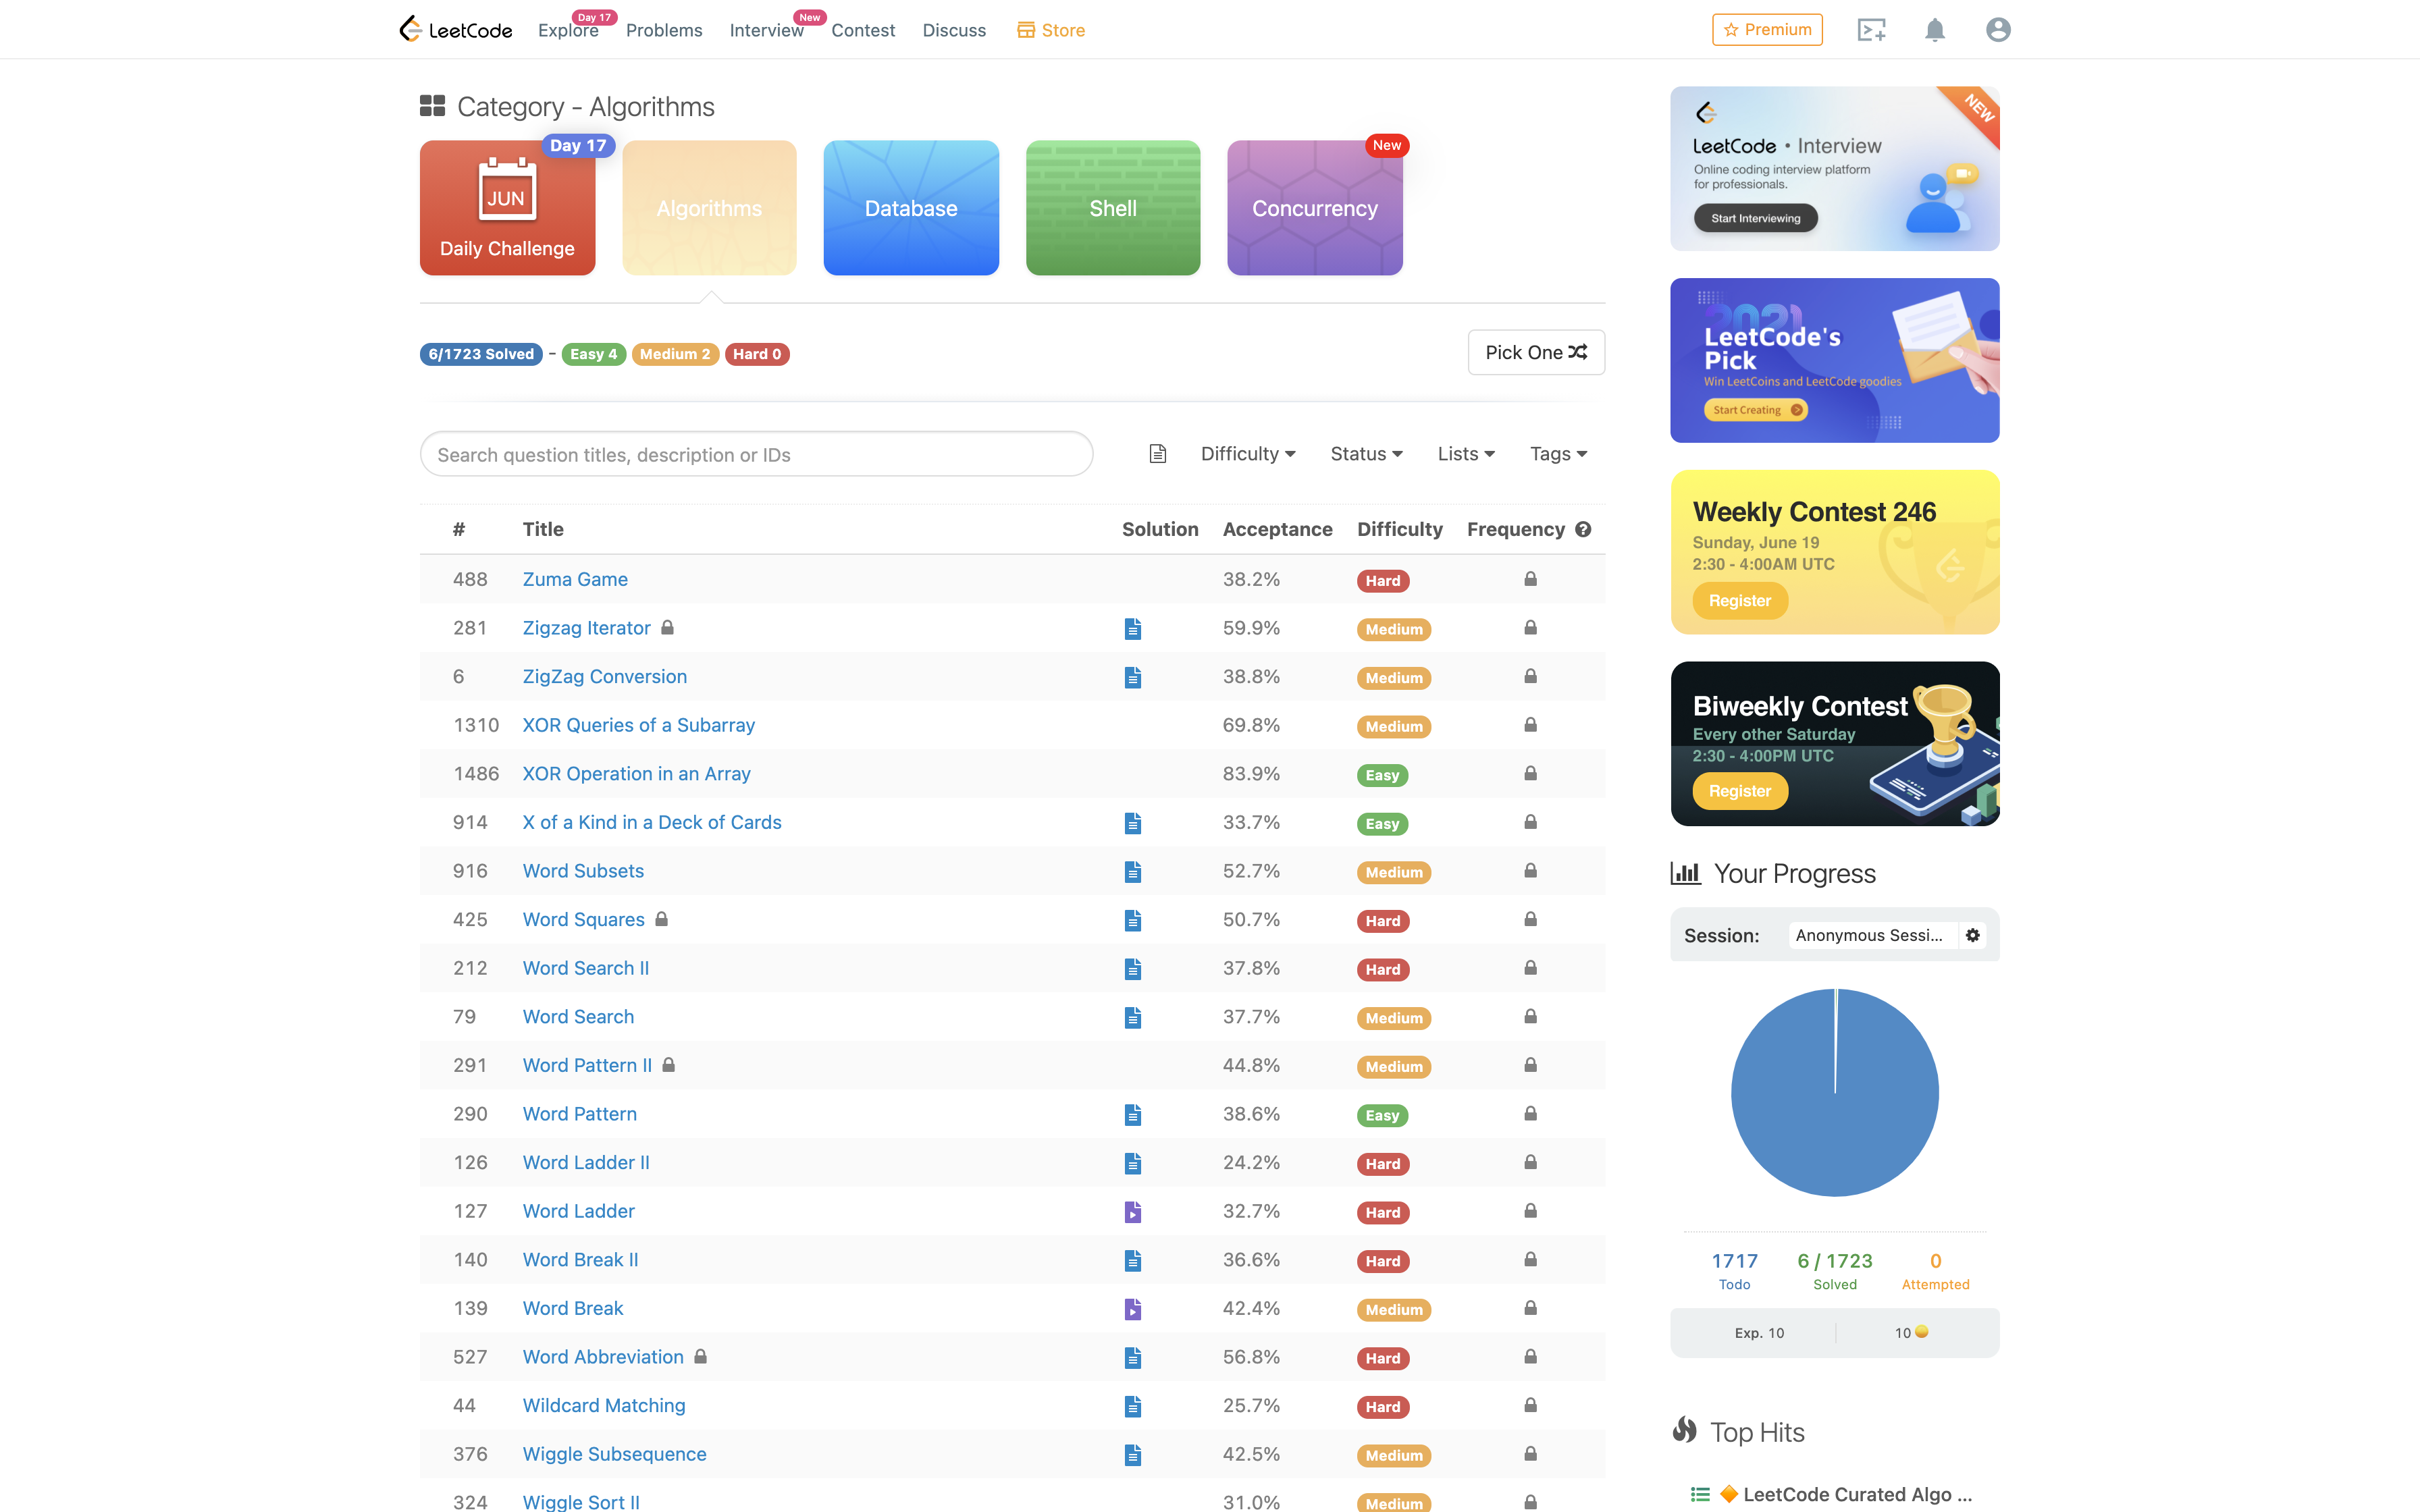
\includegraphics[width=\textwidth]{images/leetcode-ui.png}
	\caption{
		Sučelje \textit{web} aplikacije LeetCode.
	}
	\label{fig:leetcode-ui}
\end{figure}

\chapter{Analiza performansi sustava za udaljeno izvršavanje programskog kôda}
\label{chap:analysis}
Analiza performansi sustava za udaljeno izvršavanje programskog kôda se ne spominje u literaturi budući da se tek od \citep{9245310} sustavi za udaljeno izvršavanje programskog kôda razmatraju kao zasebne komponente u arhitekturi sustava za udaljeno ocjenjivanje.
\citep{drung2011enhance} razmatraju optimizaciju performansi postojećeg sustava za udaljeno ocjenjivanje, međutim, njihovo istraživanje usmjereno je u ugađanje opcija operacijskog sustava i algoritama raspoređivanja zadataka za izvršavanje.

Ovaj rad predstavlja novi radni okvir za analizu performansi sustava za udaljeno izvršavanje programskog kôda koji je nezavisan o sustavu koji se testira. Prema \citep{nidhra2012black} ovakva vrsta analize u spektru testiranja softvera naziva se \textit{system testing}, a proučava kako sustav funkcionira u produkcijskom okruženju iz perspektive korisnika. Također, prema uvidu koji imamo u sustav koji testiramo ovakva vrsta testiranja, a koja se razmatra u ovom radu, naziva se \textit{black box testing}.

Radni okvir analize performansi sustava za udaljeno izvršavanje programskog kôda (u daljnjem tekstu: \textit{radni okvir} i \textit{sustav}) sastoji se od nekoliko dimenzija kroz koje možemo promatrati performanse sustava. Kratki uvodi u svaku dimenziju slijede u nastavku ove cjeline, a nakon toga slijedi detaljni pregled svake dimenzije.

\subsubsection{Višekorisničko okruženje}
Prilikom analize u radnom okviru možemo mijenjati broj korisnika $N$ koji istovremeno stvaraju zahtjeve za izvršavanje programskog kôda. Osim broja korisnika koji istovremeno stvaraju zahtjev možemo promatrati i dinamiku kojom ti zahtjevi dolaze u sustav. Tako možemo govoriti o \textbf{impulsnom opterećenju} sustava gdje $N$ korisnika $M$ puta istovremeno napravi zahtjev za izvršavanje. U impulsnom opterećenju govorimo dakle o $M$ impulsa amplitude $N$. Impulsno opterećenje sustava u radnom okviru zahtjeva da impuls $M$ ne može započeti dok impuls $M-1$ ne završi. Na kraju impulsnog opterećenja u sustav je pristiglo $N \times M$ zahtjeva.

Za razliku od implusnog opterećenja, \textbf{kontinuirano opterećenje} sustava dozvoljava da impuls $M$ započne dok impuls $M-1$ traje, uz ogradu da se impuls $M$ smije dogoditi tek u vremenu $t_{M} = t_{M-1} + 1$, gdje je vrijeme $t$ izraženo u sekundama. Stoga, odabirom kontinuiranog opterećenja od $N$ korisnika, $M$ opet predstavlja broj impulsa, ali i vrijeme (u sekundama) trajanje eksperimenta. U sustavu će ponovo pristići $N \times M$ zahtjeva, međutim, drugačijom dinamikom nego kod impulsnog opterećenja.

Kontinuirano opterećenje sustava možemo podijeliti na determinističko i stohastičko. \textbf{Determinističko kontinuirano opterećenje} prethodno je opisano kontinuirano opterećenje gdje $N$ korisnika istovremeno stvara zahtjeve svake sekunde u ukupnom trajanju od $M$ sekundi. \textbf{Stohastičko kontinuirano opterećenje} svake sekunde u ukupnom trajanju od $M$ sekundi stvara $N_t$ korisnika gdje $N_t$ dolazi iz Poissonove distribucije s parametrima $\lambda = N$.

\subsubsection{Scenariji izvršavanja i programski jezici}
Prilikom pokretanja eksperimenta potrebno je definirati koji programski kôd će svaki korisnik koristiti. U okviru ovog rada promatraju se:
\begin{itemize}
    \item osnovni scenarij
    \item scenarij procesnog opterećenja
    \item scenarij mrežnog opterećenja
    \item scenarij procesnog i mrežnog opterećenja
\end{itemize}

Svaki scenarij implementiran je u tri različita programska jezika: Python, \text{C++} i Java. Iz toga slijedi da je na raspolaganju 12 različitih programskih kôdova koje možemo izvršavati i uspoređivati.

\subsubsection{Strategija izvršavanja}
Postoje dvije strategije izvršavanja programskog kôda koje sustavi za udaljeno izvršavanje programskog kôda podržavaju: asinkrono i sinkrono izvršavanje. Kod asinkronog izvršavanja korisnik nakon prvog zahtjeva za izvršavanjem kao rezultat dobiva jedinstveni ključ \engl{token} s kojim može asinkrono provjeravati rezultat izvršavanja. Korisnik je odgovoran za provjeru rezultata, a svaki sustav na svoj način definira kada korisnik može smatrati da je njegovo izvršavanje završilo. Kod sinkronog izvršavanja korisnik kao rezultat zahtjeva dobiva rezultat izvršavanja.

\subsubsection{Sustav za izvršavanje}
Prilikom pokretanja eksperimenta potrebno je odrediti koji sustav želimo testirati. U okviru ovog rada promatraju se tri vrste sustava: Sphere Engine, Piston i Judge0, međutim, omogućeno je da se promatraju različite instance svake vrste sustava.

\section{Simulacija višekorisničkog opterećenja}
Budući da sustav za udaljeno izvršavanje programskog kôda neposredno preko sustava za udaljeno ocjenjivanje koristi više korisnika istovremeno, u analizi performansi potrebno je razmatrati višekorisničko opterećenje.

Radni okvir omogućuje razmatranje tri različite vrste višekorisničkog opterećenja koje se koriste prilikom stvaranja zahtjeva za izvršavanjem programskog kôda (u nastavku teksta: \textit{zahtjevi}):
\begin{itemize}
    \item impulsno-determinističko opterećenje,
    \item kontinuiran-determinističko opterećenje, i
    \item kontinuirano-stohastičko opterećenje.
\end{itemize}

Svaka vrsta višekorisničkog opterećenja detaljno je opisana u nastavku.

\subsection{Impulsno-determinističko opterećenje sustava}
Impulsno-determinističko opterećenje sustava definirano je parametrima $N$ i $M$ gdje $N$ predstavlja broj zahtjeva koje treba poslati istovremeno, a $M$ predstavlja broj iteracija koje je potrebno napraviti uz ogradu da zahtjevi poslani u iteraciji $i$ smiju biti poslani tek nakon što se izvrše zahtjevi u iteraciji $i - 1$. U svakoj od $M$ iteracija poslat će se $N$ zahtjeva istovremeno, odnosno, na kraju eksperimenta opterećenja u sustav je pristiglo ukupno $N \times M$ zahtjeva za izvršavanje.

\begin{figure}[htb]
	\centering
	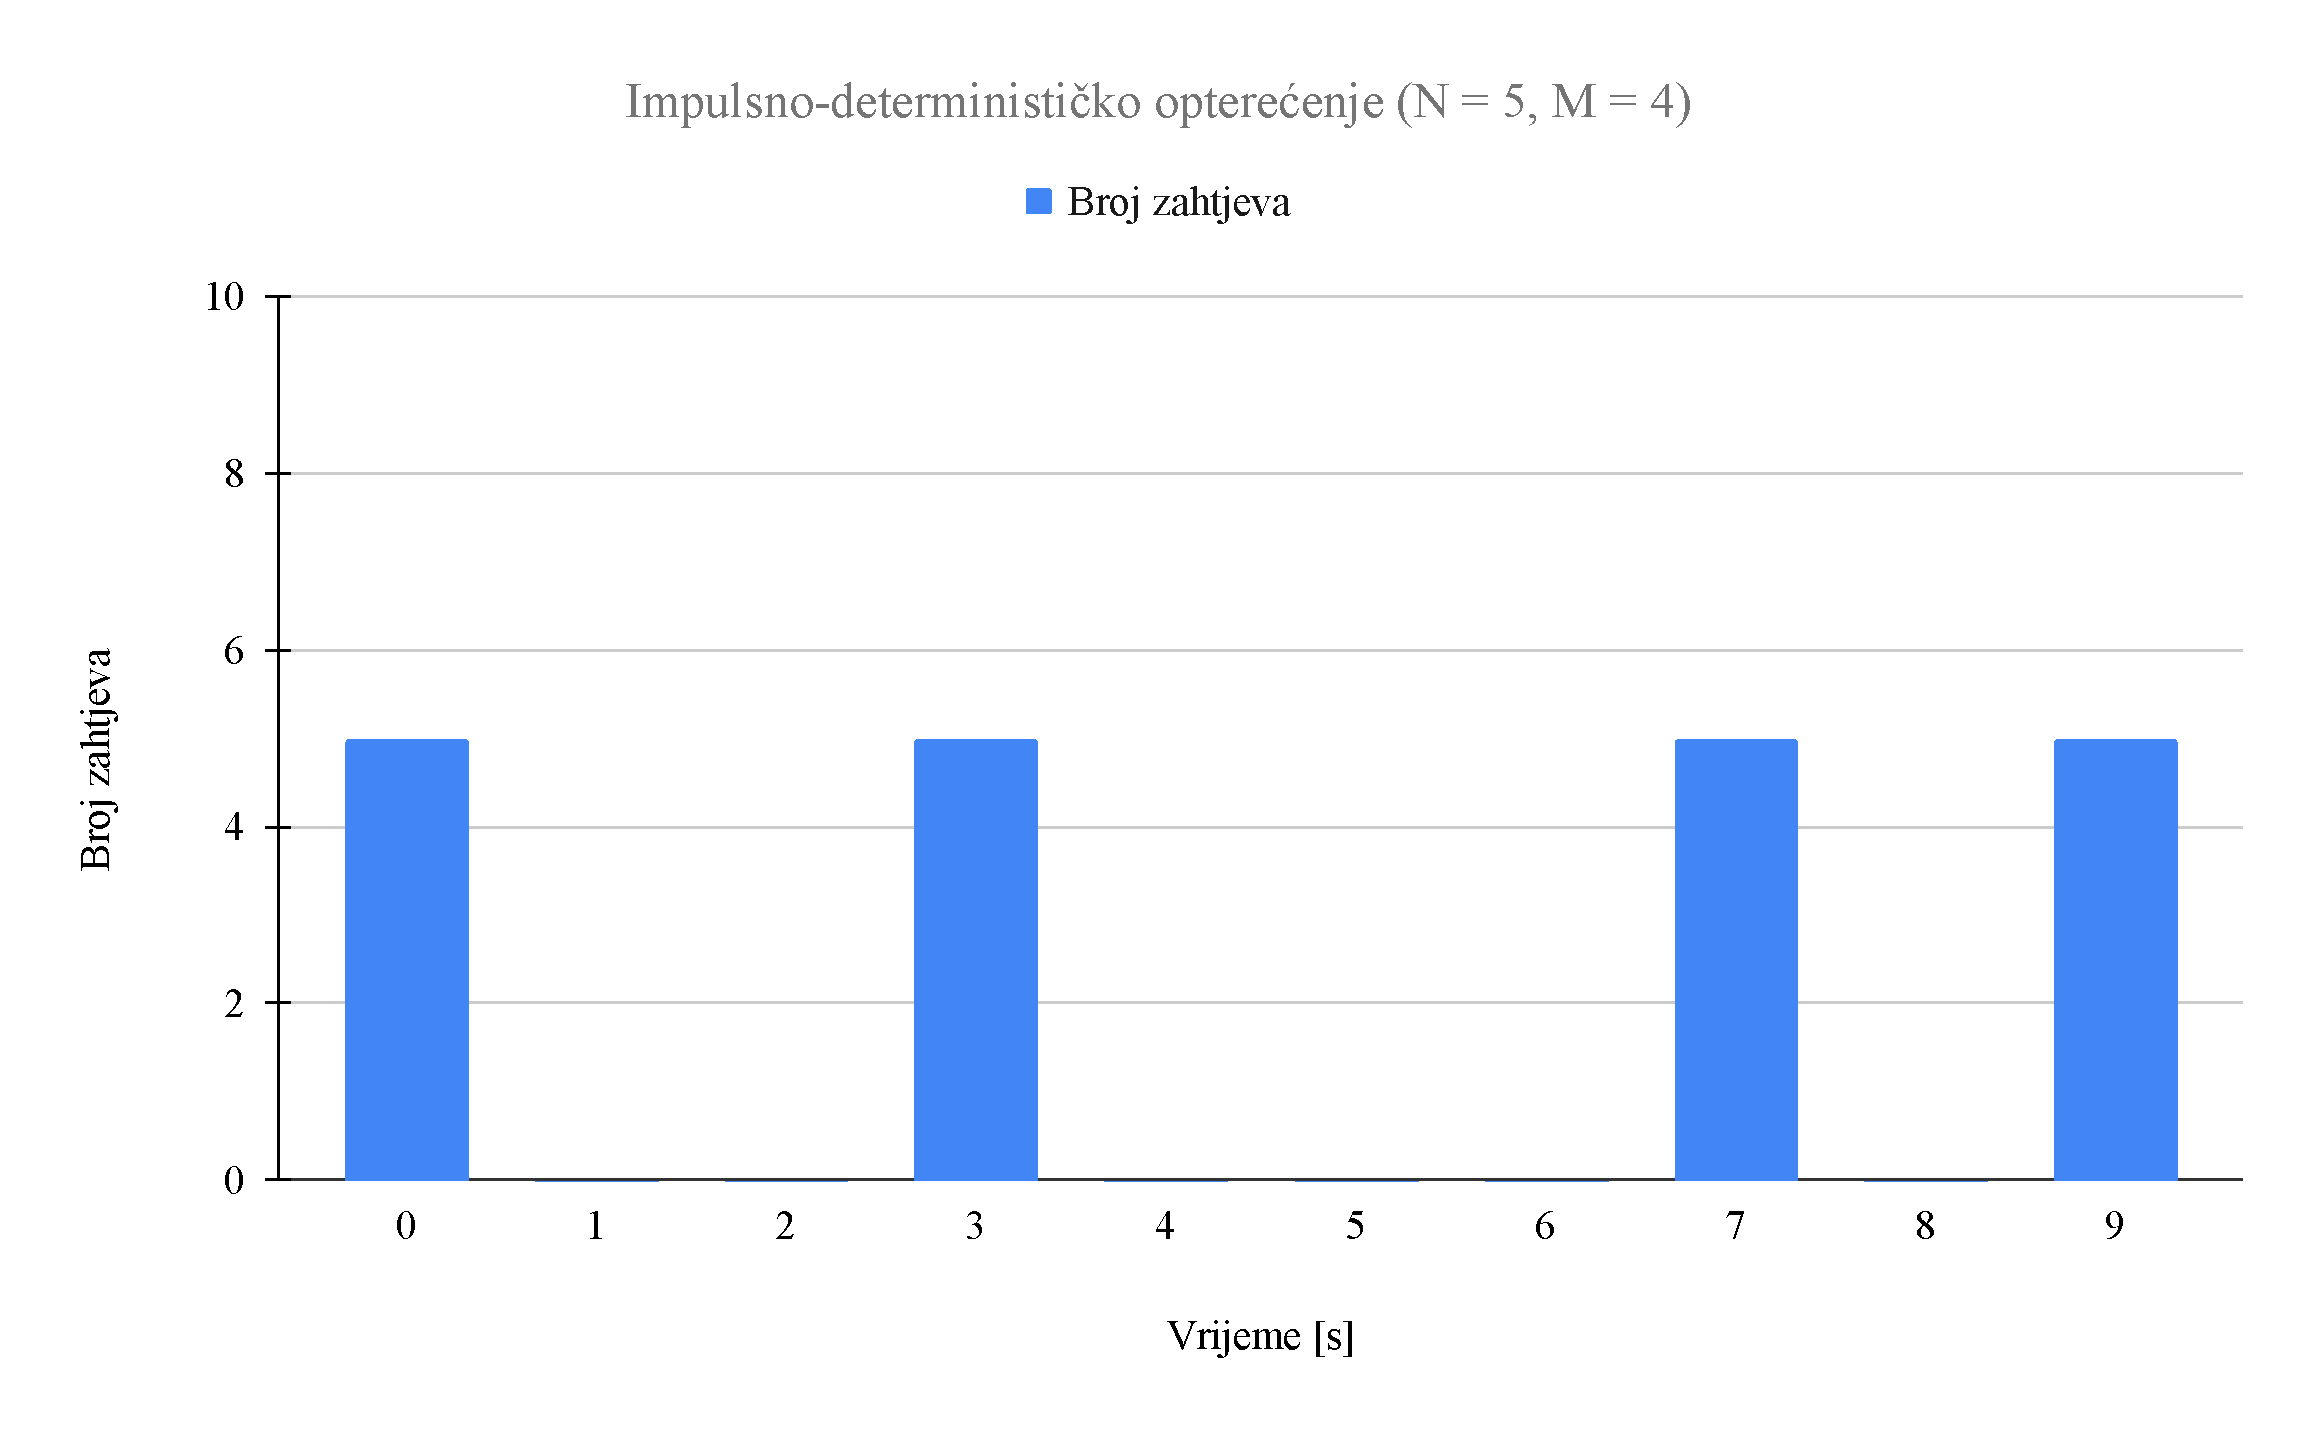
\includegraphics[width=\textwidth]{images/Impulsno-determinističko opterećenje (N = 5, M = 4).pdf}
	\caption{
		Impulsno-determinističko opterećenje sustava (N = 10, M = 6).
	}
	\label{fig:impulse-load}
\end{figure}

Slika \ref{fig:impulse-load} prikazuje primjer dinamike impulsno-determinističkog opterećenja sustava. U ovom primjeru koristi se 6 impulsa amplitude 10, odnosno, 6 puta se šalje 10 istovremenih zahtjeva za izvršavanje. Slika također prikazuje da je trećem impulsu zahtjeva potrebno 2 sekunde više za izvršavanje nego što je to bilo impulsima 1 i 2. Ovakav primjer odabran je kako bi se naglasilo svojstvo disjunktnosti susjednih impulsa. Interpretacija rezultata ovog primjera i objašnjenje zbog čega može doći do pomaka u vremenu izvršavanja ostavlja se za raspravu.

\subsection{Kontinuirano-determinističko opterećenje sustava}
Kontinuirano-determinističko opterećenje sustava definirano je također parametrima $N$ i $M$, međutim, za razliku od prethodne vrste opterećenja sustava, ograda ove vrste opterećenja jest da istovremeni zahtjevi u iteraciji $i$ mogu započeti tek u vremenu $t_i = t_{i - 1} + 1$, gdje je $t$ vrijeme izraženo u sekundama.

\begin{figure}[htb]
	\centering
	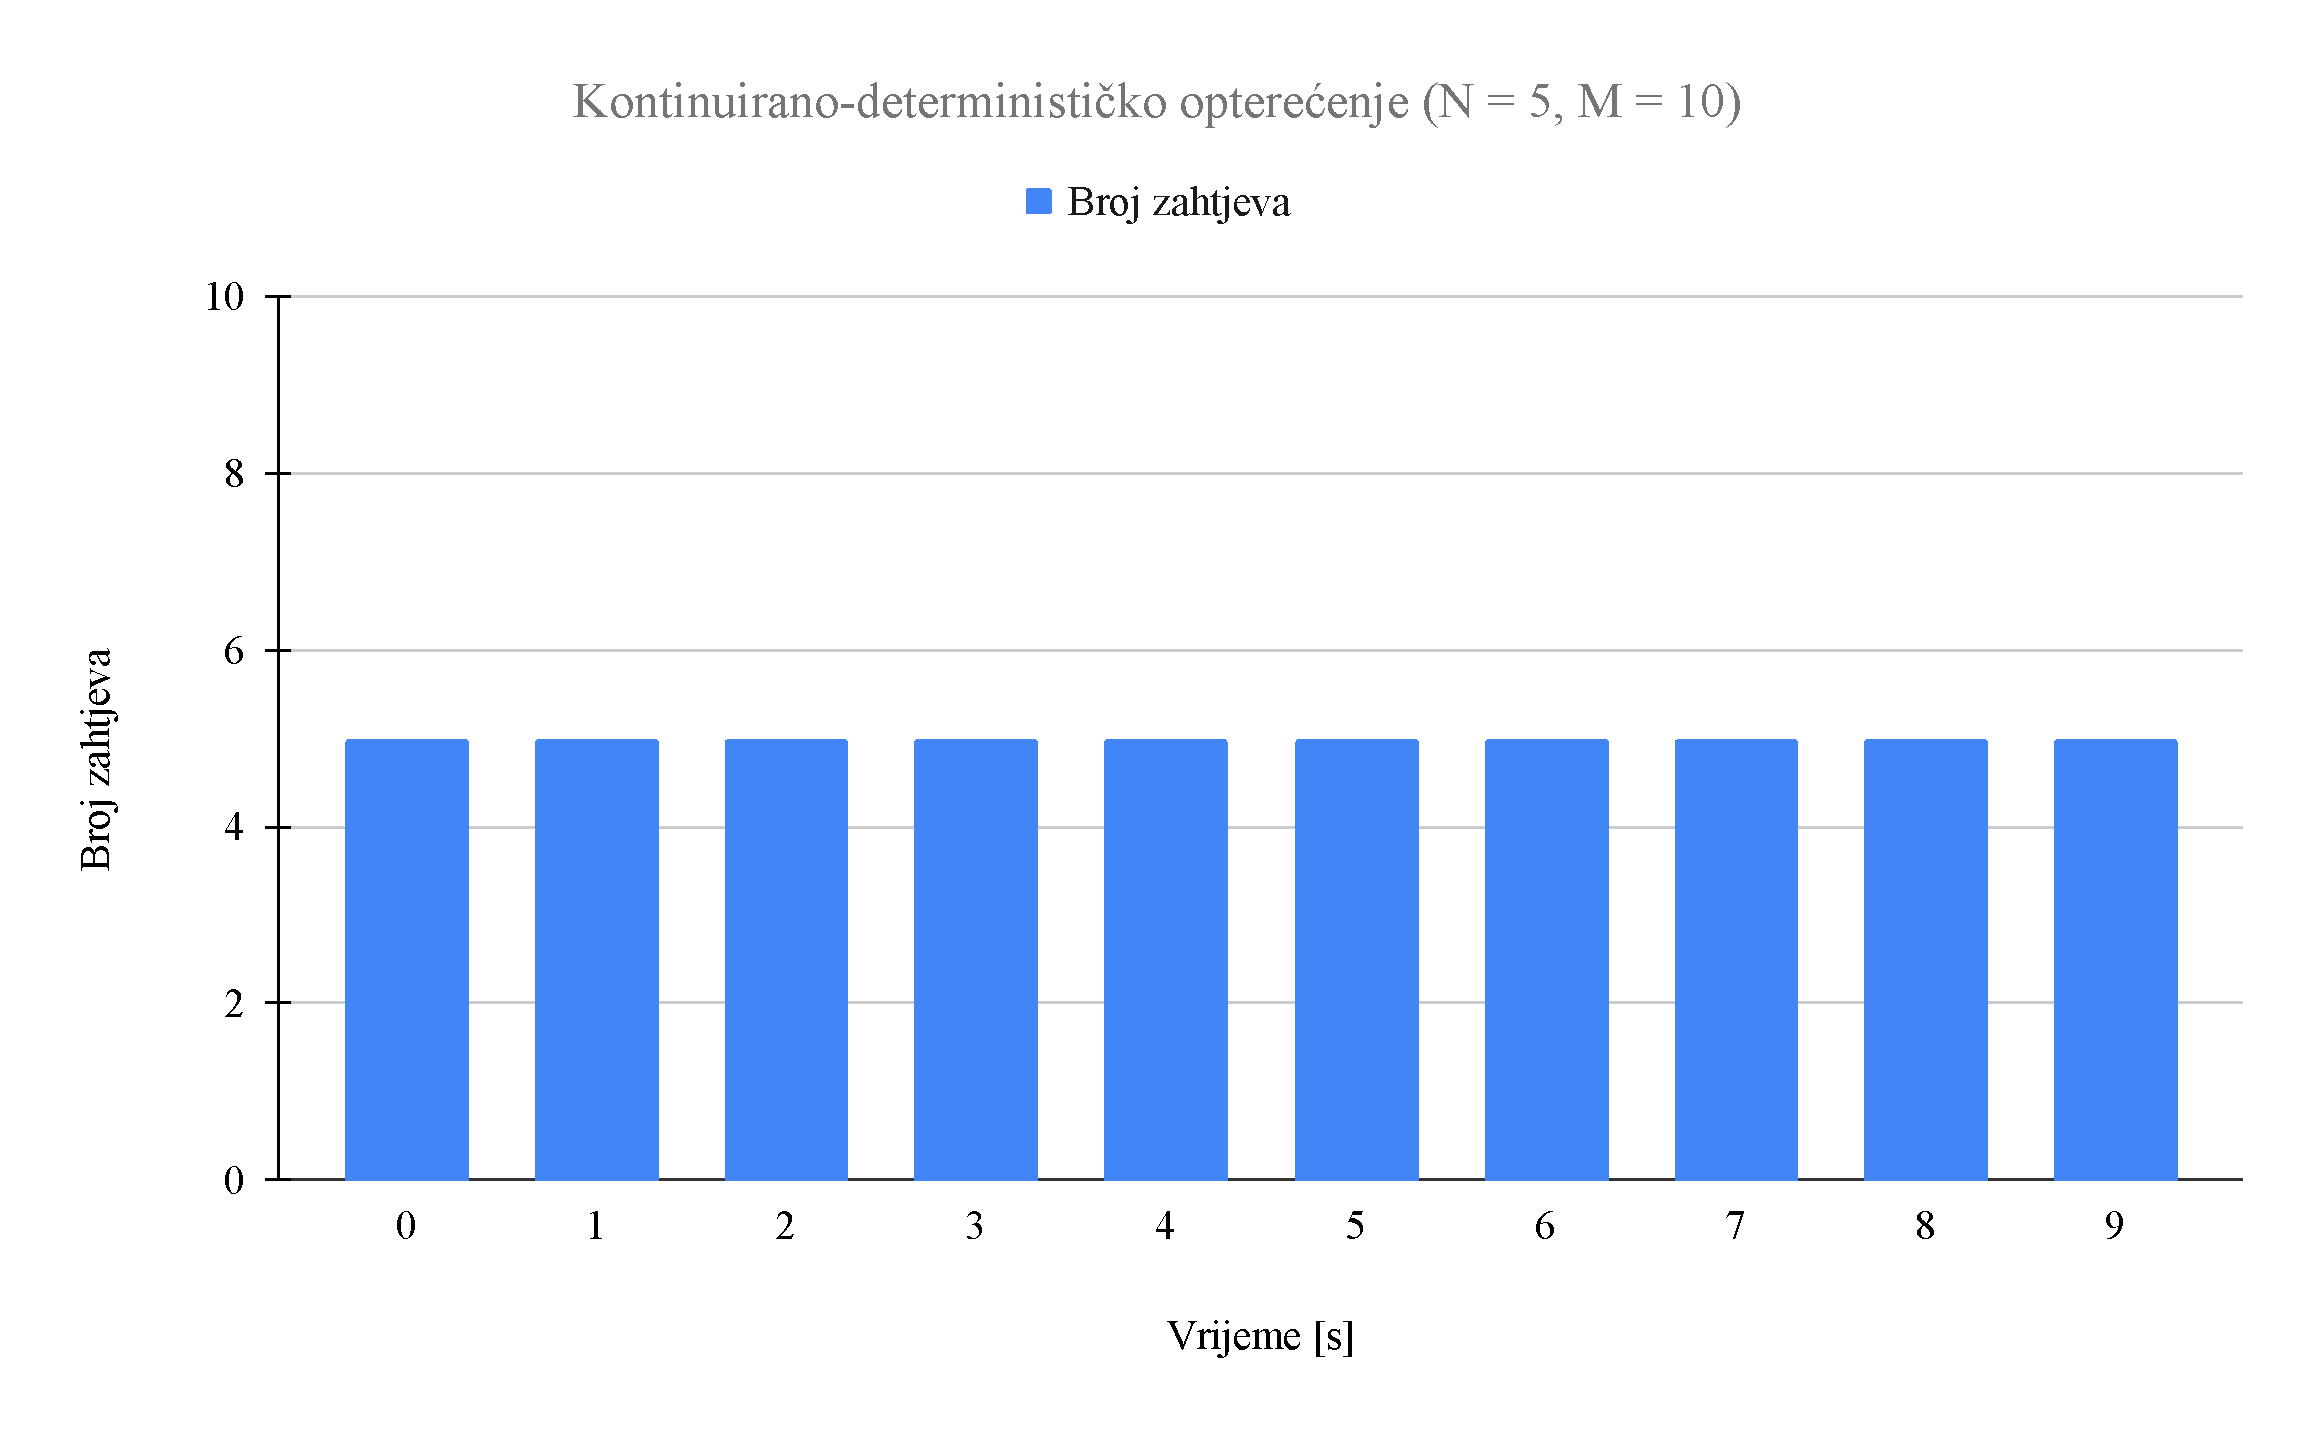
\includegraphics[width=\textwidth]{images/Kontinuirano-determinističko opterećenje (N = 5, M = 10).pdf}
	\caption{
		Kontinuirano-determinističko opterećenje sustava (N = 10, M = 20).
	}
	\label{fig:deterministic-load}
\end{figure}

\subsection{Kontinuirano-stohastičko opterećenje sustava}
Kontinuirano-stohastičko opterećenje sustava koristi Poissonovu distribuciju s parametrom $\lambda = N$ za određivanje broja istovremenih zahtjeva u koraku $i$. Slika \ref{fig:stochastic-load} prikazuje primjer dinamike dolaska zahtjeva u sustav koristeći kontinuirano-stohastičko opterećenje s parametrima $N=10$ i $M=20$. Niz pseudo-slučajnih brojeva sa slike \ref{fig:stochastic-load} generiran je pomoću isječka \ref{lst:poisson-numbers} napisanog u Python programskog jeziku.

\begin{figure}[htb]
	\centering
	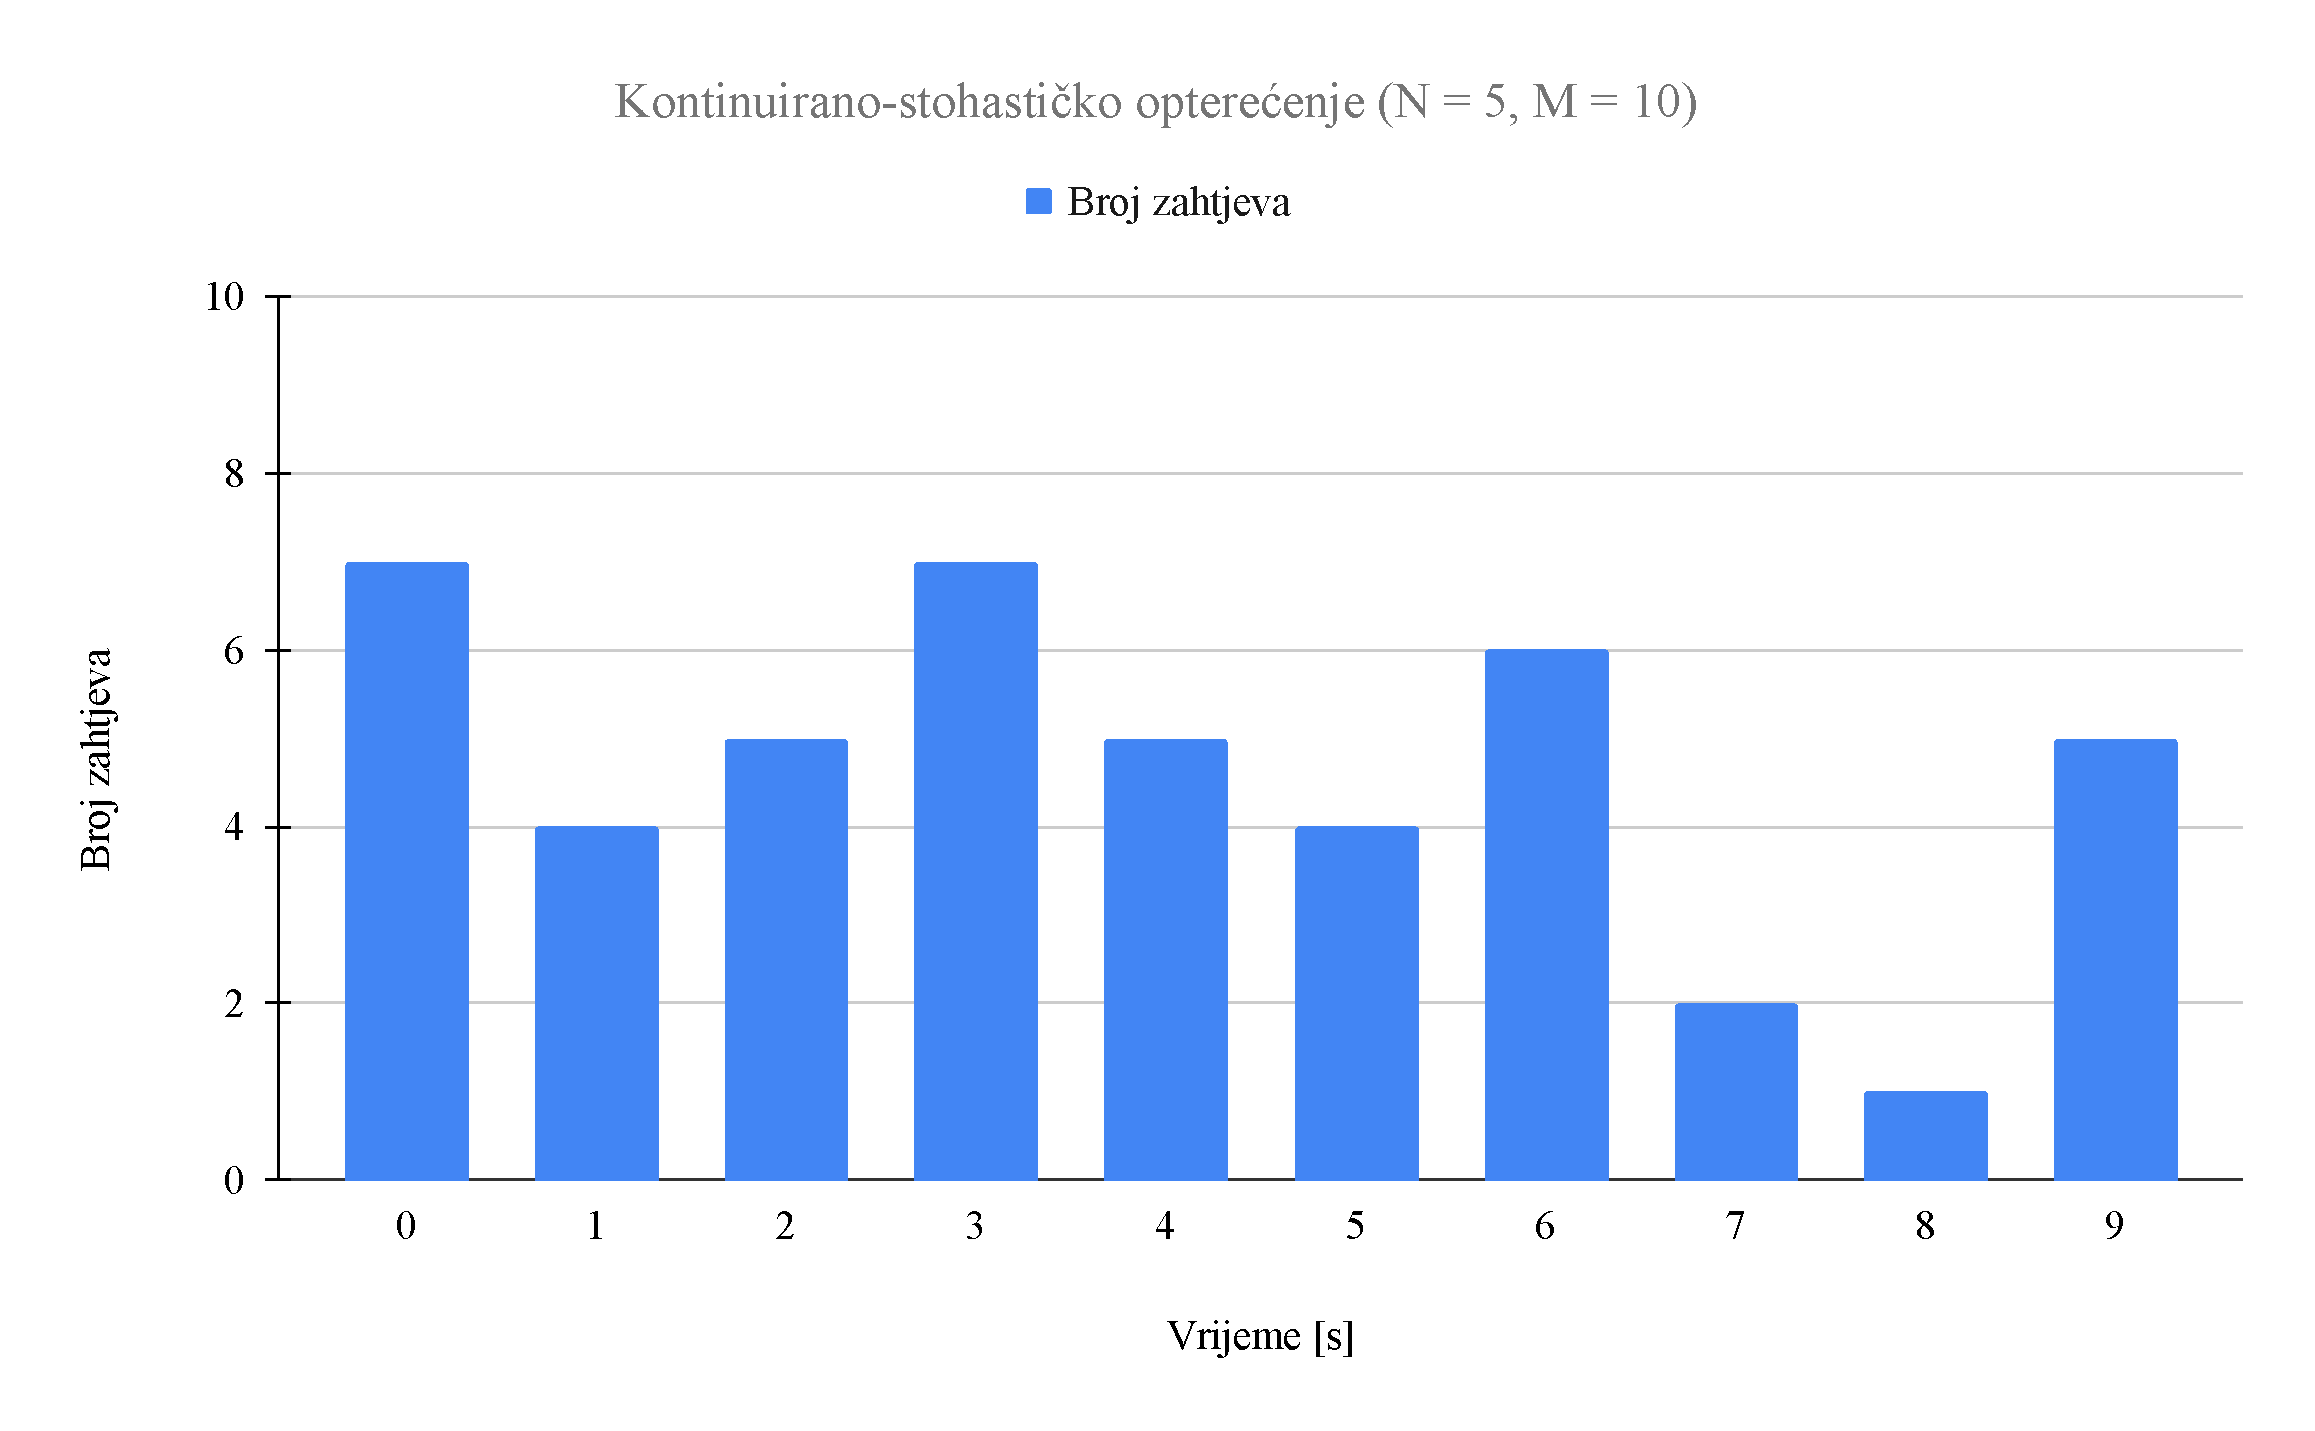
\includegraphics[width=\textwidth]{images/Kontinuirano-stohastičko opterećenje (N = 5, M = 10).pdf}
	\caption{
		Kontinuirano-stohastičko opterećenje sustava (N = 10, M = 20).
	}
	\label{fig:stochastic-load}
\end{figure}

\begin{lstlisting}[
    caption={Generiranje pseudo-slučajnih brojeva iz Poissonove distribucije.},
    label={lst:poisson-numbers},
    language=python
]
import numpy
N, M = 5, 10
print(numpy.random.poisson(N, M))
\end{lstlisting}

\section{Korisnički scenariji i programski jezici}
Korisnički scenariji definiraju obrazac korištenja sustava za udaljeno izvršavanje programskog kôda. U produkcijskom okruženju nemoguće je predvidjeti koji programski kôd će sustav trebati izvesti, međutim, u svrhu analize sustava za udaljeno izvršavanje programskog kôda programi koji pristižu u sustav mogu se podijeliti u četiri osnovne kategorije: osnovni scenarij, scenarij procesnog opterećenja, scenarij mrežnog opterećenja, scenarij procesnog i mrežnog opterećenja.

Svaki scenarij zapravo je pažljivo odabrani zadatak koji korisnik treba riješiti, međutim, za razliku od uobičajenih zadataka, scenarij daje uputu na koji način zadatak treba riješiti. Ova ograda važna je da bi se mogla raditi analiza između dva različita scenarija. Tako se npr.\ uz pažljivo odabrane scenarije mogu uspoređivati scenarij procesnog opterećenja, i scenarij procesnog i mrežnog opterećenja samo ako se zna da je drugi zaista mrežno opterećena inačica prvog.

Prilikom analize pretpostavlja se da su programski kôdovi scenarija ispravni, odnosno da se mogu uspješno prevesti i izvesti u svakom sustavu koji se promatra. Ova pretpostavka uspješnosti prevođenja i izvršavanja ključna je u analizi budući da u višekorisničkom opterećenju može doći do preopterećenja sustava koje rezultira npr. u neuspješnom prevođenju zbog manjka radne memorija. Pregled razloga neuspješnih izvršavanja bit će opisani u analizi performansi pojedinih sustava.

Implementacija svakog korisničkih scenarija dostupna je u tri programska jezika: \text{C++}, Java i Python. Iako se u okviru ovog rada promatraju samo navedeni programski jezici, radni okvir analize nije ograničen samo na njih. Također u ovom radu ne razmatraju se višedretvene implementacije scenarija.

Svaki scenarij sastoji se od: sadržaja standardnog ulaza, programskog kôda i očekivanog standardnog izlaza. Standardni ulaz i očekivani standardni izlaz programa isti je za svaki programski jezik u kojem je scenarij napisan. Sadržaj standardnog ulaza dovodi se na ulaz programa koji je nastao prevođenjem programskog kôda scenarija u odabranom programskom jeziku, a očekivani standardni izlaz koristi se za usporedbu sa standardnim izlazom programa nakon njegovog izvršavanja. Ova provjera važna ja kako bi se utvrdilo da je program zaista odradio zadatak zadan scenarijem.

\subsection{Osnovni scenarij}
Osnovni scenarij zahtjeva da korisnički program na standardni izlaz ispiše ``\textit{hello, world}''. Sadržaj standardnog ulaza ovog scenarija ne sadrži ništa, dok očekivani standardni izlaz programa sadrži niz znakova ``\textit{hello, world}''.

Osnovni scenarij predstavlja najjednostavniji smisleni programski kôd koji korisnik može izvesti putem sustava. Ovaj scenarij također predstavlja minimalno mrežno, procesno i memorijsko opterećenje na poslužitelju sustava.

Vremenska i memorijska složenost algoritma koji implementira rješenje ovog scenarija je $\mathcal{O}(1)$.

\subsection{Scenarij procesnog opterećenja}
Scenarij procesnog opterećenja zahtjeva ispis medijana od 20000 cijelih brojeva tipa \textit{integer} koji na standardni ulaz dolaze silazno sortirani. Scenarij također zahtjeva da se pročitanih 20000 brojeva najprije uzlazno sortira mjehurićastim sortiranjem \engl{bubble sort}.

Vremenska složenost algoritma koji implementira rješenje ovog scenarija je $\mathcal{O}(n^2)$, a memorijska složenost je $\mathcal{O}(n)$, gdje je $n$ duljina ulaznog niza brojeva.

Odabir 20000 za duljinu ulaznog niza brojeva i zahtjev da brojevi budu sortirani suboptimalnim algoritmom mjehurićastog sortiranja nije slučajan, nego pažljivo odabran budući da vrijeme izvođenja programa koji implementira rješenje tog scenarija traje zamjetno dulje od osnovnog scenarija. Konkretno, na procesoru Intel Core i7 radnog takta 2.6 GHz računala MacBook Pro (16-inch, 2019) \text{C++} implementacija rješenja ovog scenarija traje oko 2.5 sekundi.

Ulazni niz brojeva koji na standardni ulaz dolaze silazno sortirani odabran je zato što to predstavlja najgori slučaj \engl{worst case} za algoritam mjehurićastog sortiranja koji brojeve treba sortirati uzlazno.

\subsection{Scenarij mrežnog opterećenja}
Scenarij mrežnog opterećenja očekuje da program ispiše sumu 750000 cijelih brojeva tipa \textit{integer} koji na standardni ulaz dolaze silazno sortirani.

Mrežno opterećenje ovog scenarija očituje se u veličini sadržaja standardnog ulaza kojeg je poterbno dovesti programu, a ono iznosi 5.1 MB.

Vremenska i memorijska složenost algoritma koji implementira rješenje ovog scenarija je $\mathcal{O}(n)$, gdje je $n$ duljina ulaznog niza brojeva.

\subsection{Scenarij procesnog i mrežnog opterećenja}
Scenarij procesnog i mrežnog opterećenja kombinacija je prethodna dva scenarija. Ovaj scenarij zahtjeva da program ispiše medijan od prvih 20000 brojeva iz niza od 750000 brojeva koji na standardni ulaz dolaze silazno sortirani. Također, kao i u scenariju procesnog opterećenja, od programa se očekuje da brojeve sortira suboptimalnim algoritmom mjehurićastog sortiranja.

Standardni ulaz ovog scenarija isti je kao i standardni ulaz scenarija mrežnog opterećenja, i algoritam rješenja ovog scenarija isti je kao algoritam rješenja scenarija procesnog opterećenja.

Vremenska složenost algoritma koji implementira rješenje ovog scenarija je $\mathcal{O}(n^2)$, a memorijska složenost je $\mathcal{O}(n)$, gdje je $n$ duljina ulaznog niza brojeva, uz ogradu da $n$ ne može biti veći od 20000.

\section{Strategije izvršavanja}
Zahtjev za izvršavanje programskog kôda može se napraviti na dva načina: sinkrono i asinkrono. Slika \ref{fig:sync-execution} prikazuje dijagram toka sinkronog izvršavanja programskog kôda. Korisnik započinje interakciju s sustava stvarajući zahtjev za izvršavanjem, zatim sustav kao odgovor vraća korisniku rezultate izvršavanja. Budući da izvršavanje programskog kôda može trajati i po nekoliko sekundi ova strategija izvršavanja može iscrpiti poslužiteljske resurse prilikom intenzivnog višekorisničkog opterećenja.

\begin{figure}[htb]
	\centering
	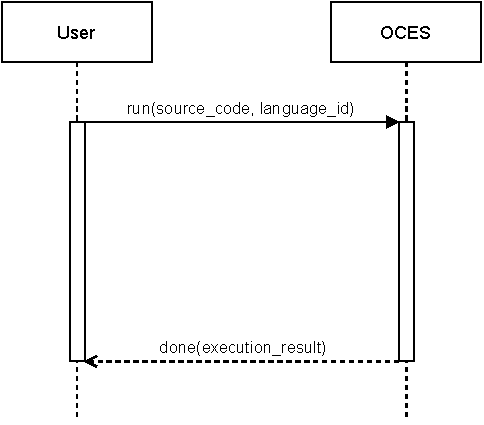
\includegraphics[width=0.75\textwidth]{images/sync-execution.pdf}
	\caption{
		Sinkrono izvršavanje programskog kôda.
	}
	\label{fig:sync-execution}
\end{figure}

Asinkrono izvršavanje programskog kôda započinje na isti način kao i sinkrono - stvaranjem zahtjeva za izvršavanje, međutim, u asinkronoj strategiji sustav korisniku vraća jedinstveni identifikator zahtjeva kojeg je korisnik napravio. Nakon toga korisnik treba posebnim zahtjevom provjeravati status svog zahtjeva dok ne utvrdi da je izvršavanje završilo.

\begin{figure}[htb]
	\centering
	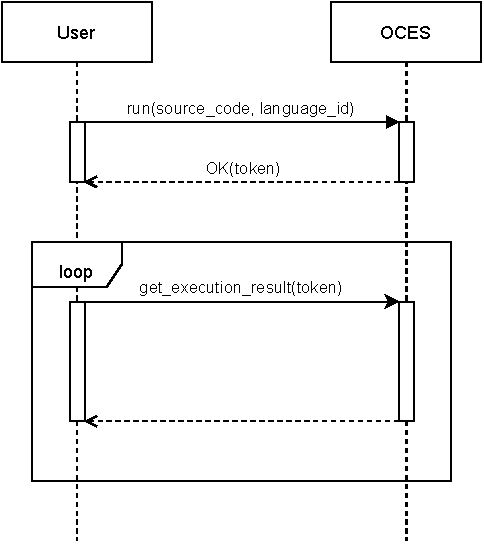
\includegraphics[width=0.75\textwidth]{images/async-execution.pdf}
	\caption{
		Asinkrono izvršavanje programskog kôda.
	}
	\label{fig:async-execution}
\end{figure}

\section{Metrike za analizu performansi}
Radni okvir analize performansi sustava za udaljeno izvršavanje programskog kôda razmatra dvije metrike: uspješnost izvođenja i vrijeme obrade.

\subsubsection{Uspješnost izvršavanja}
Budući da prilikom intenzivnog višekorisničkog opterećenje može doći do preopterećenja sustava, zahtjevi za izvršavanje mogu biti odbačeni ili može doći do greške uslijed prevođenja ili izvršavanja zbog manjka slobodnih resursa na poslužitelju sustava. Ovo su samo neki od brojnih razloga zbog čega sustav može neuspješno izvršiti programski kôd korisnika i razmatranje svakog pojedinog razloga izlazi iz opsega ovog rada. Također, za potpuno razumijevanje neuspješnog izvršavanja potrebno je imati uvid u sustav koji se analizira, međutim, radni okvir analize koju ovaj rad predlaže podrazumijeva tzv.\ \textit{black box} pristup.

\subsubsection{Vrijeme obrade}
Vrijeme obrade \engl{turn around time} najvažnija je metrika iz perspektive krajnjeg korisnika. Iz perspektive krajnjeg korisnika sustava za udaljeno ocjenjivanje vrijeme obrade je vrijeme koje je potrebno da korisnik na zaslonu dobije rezultat izvršavanja svog programa. Budući da sustav za udaljeno izvršavanje programskog kôda korisnici ne koriste direktno, nego neposredno preko sustava za udaljeno ocjenjivanje, korisnikom sustava za udaljeno izvršavanje programskog kôda smatra se sustav za udaljeno ocjenjivanje.

Vrijeme obrade programskog kôda definira se kao proteklo vrijeme između trenutka kada je korisnik zahtjevom za izvršavanjem poslao sve podatke potrebne sustavu, do trenutka kada je korisnik ustanovio da je izvršavanje završilo.

\chapter{Aplikacija Hélory}
\label{chap:helory}
Aplikacija Hélory prva je specijalizirana aplikacija za višekorisničko opterećenje i analizu performansi sustava za udaljeno izvršavanje programskog kôda. Komandno-linijsko sučelje aplikacije Hélory omogućuje korisnicima pokretanje višekorisničkog opterećenja na tri različita sustava za udaljeno izvršavanje programskog kôda: Sphere Engine, Piston i Judge0.

Kao rezultat eksperimentalnog višekorisničkog opterećenja Hélory u tekućem direktoriju pohranjuje izvještaj u HTML formatu koji sadrži sve relevantne informacije o eksperimentu, grafički prikaz metrika od interesa i sirove podatke u formatu JSON prikupljene za vrijeme eksperimenta koji naknadno mogu biti dodatno iskorišteni.

\section{Korištene tehnologije}
Hélory je razvijen u statičkom i tipiziranom programskom jeziku Go \citep{donovan2015go} koji se brzo prevodi u strojni kôd i kojeg odlikuje ekspresivnost, preciznost, jednostavnost i čistoća u pisanju programskog kôda, i jednostavnost pisanja konkuretnih programa koji efikasno iskorištavaju resurse domaćina. Izvještaj kojeg generira Hélory nakon eksperimenta napisan je u opisnom jeziku HTML uz korištenje CSS-a i JavaScripta, a za prikaz metrika od interesa u grafičkom obliku koristi se biblioteka Chart.js\footnote{https://github.com/chartjs/Chart.js}.

\section{Prikupljanje podataka}
Isječak \ref{lst:json-report} prikazuje primjer sirovih podataka u formatu JSON koje je sustav Hélory prikupio za vrijeme eksperimenta. Značenje svakog pojedinog ključa je sljedeće:
\begin{itemize}
    \item[$\bullet$] \lstinline{id} - jedinstveni identifikator,
    \item[$\bullet$] \lstinline{name} - ime eksperimenta,
    \item[$\bullet$] \lstinline{started_at} - vremenski trenutak početka,
    \item[$\bullet$] \lstinline{finished_at} - vremenski trenutak završetka,
    \item[$\bullet$] \lstinline{scenario} - korišteni scenarij,
    \item[$\bullet$] \lstinline{scenario_description} -- opis korištenog scenarija,
    \item[$\bullet$] \lstinline{language} - korišteni programski jezik,
    \item[$\bullet$] \lstinline{endpoint} - ime korištenog sustava za udaljeno izvršavanje programskog kôda,
    \item[$\bullet$] \lstinline{endpoint_url} - poveznica na korišteni sustav za udaljeno izvršavanje programskog kôda,
    \item[$\bullet$] \lstinline{strategy} - korištena strategija izvršavanja programskog kôda,
    \item[$\bullet$] \lstinline{experiment_type} - vrsta višekorisničkog opterećenja,
    \item[$\bullet$] \lstinline{experiment_configuration} - konfiguracijske opcije specifične za vrstu višekorisničkog opterećenja, i
    \item[$\bullet$] \lstinline{executions} - niz rezultata izvršavanja programskog kôda.
\end{itemize}

Jedinstveni identifikator eksperimenta \lstinline{id} dodjeljuje se eksperimentu na temelju 
\pagebreak

\begin{lstlisting}[
    caption={Podaci o izvršavanju prikupljeni sustavom Hélory.},
    label={lst:json-report},
]
{ 
  "id": "2021-06-22T23:43:31+02:00-deterministic-cpu ...",
  "name": "CPU Intensive in C++ via Judge0 CE with ...",
  "started_at": "2021-06-22T23:43:31.863526+02:00",
  "finished_at": "2021-06-22T23:43:41.749487+02:00",
  "scenario": "CPU Intensive",
  "scenario_description": "Find median of 20k integers ...",
  "language": "C++",
  "endpoint": "Judge0 CE",
  "endpoint_url": "https://ce.judge0.com",
  "strategy": "async",
  "experiment_type": "deterministic",
  "experiment_configuration": { "users": "2", "wait": true },
  "executions": [{
      "success": true,
      "started_at": "2021-06-22T23:43:31.863754+02:00",
      "finished_at": "2021-06-22T23:43:41.749159+02:00",
      "order_started_at": "2021-06-22T23:43:31.864903+02:00",
      "order_sent_at": "2021-06-22T23:43:32.142372+02:00",
      "order_finished_at": "2021-06-22T23:43:33.968738+02:00",
      "probes_started_at": [
        "2021-06-22T23:43:35.968855+02:00",
        "2021-06-22T23:43:38.457406+02:00"
      ], "probes_finished_at": [
        "2021-06-22T23:43:37.45341+02:00",
        "2021-06-22T23:43:39.653258+02:00"
      ]
    }, {
      "success": true,
      "started_at": "2021-06-22T23:43:31.863732+02:00",
      "finished_at": "2021-06-22T23:43:39.666589+02:00",
      "order_started_at": "2021-06-22T23:43:31.864981+02:00",
      "order_sent_at": "2021-06-22T23:43:32.142418+02:00",
      "order_finished_at": "2021-06-22T23:43:33.972937+02:00",
      "probes_started_at": [
        "2021-06-22T23:43:35.973006+02:00"
      ], "probes_finished_at": [
        "2021-06-22T23:43:37.453396+02:00"
      ]
    }]
}
\end{lstlisting}

\pagebreak

\section{Pregled komandno-linijskog sučelja}
jednostavno sučelje s mnogo opcija.

\subsection{Definiranje dostupnih sustava za udaljeno izvršavanje}
\subsubsection{Podržani sustavi za udaljeno izvršavanje}
\subsubsection{Podržane strategije izvršavanja}
\subsection{Definiranje korisničkih scenarija}
\subsubsection{Datoteka korisničkog scenarija}
\subsubsection{Programski kôd}
\subsubsection{Standardni ulaz}
\subsubsection{Standardni izlaz}
\subsection{Pokretanje opterećenja sustava}
\subsubsection{Determinističko opterećenje sustava}
\subsubsection{Stohastičko opterećenje sustava}
\section{Pregled sučelja grafičkih rezultata}

\chapter{Primjer korištenja sustava Hélory}
\label{chap:use}
\section{Analiza performansi sustava Piston}
\section{Analiza performansi sustava Judge0}

\chapter{Budući razvoj}
\label{chap:future}

\chapter{Zaključak}

\bibliography{literatura}
\bibliographystyle{fer}

\begin{sazetak}
\kljucnerijeci{Ključne riječi, odvojene zarezima.}
\end{sazetak}

\engtitle{Performance analysis of online code execution systems}
\begin{abstract}
\keywords{Keywords.}
\end{abstract}

\end{document}
